\documentclass[times, 10pt,twocolumn]{article} 
\usepackage{latex8}
\usepackage{times}
\usepackage{graphicx,amsmath,comment}
\newcommand{\igH}[1]{\includegraphics[height=.9\textheight]{#1}}
\newcommand{\igW}[1]{\includegraphics[width=.9\textwidth]{#1}}
\newcommand{\igWh}[1]{\includegraphics[width=.7\textwidth]{#1}}
\newcommand{\igWhalf}[1]{\includegraphics[width=.45\textwidth]{#1}}
\newcommand{\lda}{Latent Dirichlet Allocation}
\pagestyle{empty}


\usepackage[usenames]{color}
\definecolor{changecolor1}{rgb}{0.5,0.3,0.08} 
\definecolor{changecolor2}{rgb}{0.3,0.08,0.45} 
\definecolor{changecolor3}{rgb}{0.3,0.45,0.45} 
\definecolor{changecolor4}{rgb}{0.0,0.3,0.0} 
\newcommand{\hl}[1]{{\color{changecolor1} #1 }}
\newcommand{\hla}[1]{{\color{changecolor2} #1 }}
\newcommand{\hlb}[1]{{\color{changecolor3} #1 }}
\newcommand{\hlc}[1]{{\color{changecolor4} #1 }}

% \newcommand{\hl}[1]{#1}
% \newcommand{\hla}[1]{#1}
% \newcommand{\hlb}[1]{#1}
% \newcommand{\hlc}[1]{#1}




\author{Abram Hindle, Michael Godfrey and Ric Holt \\
\{ahindle,migod,holt\}@cs.uwaterloo.ca\\
Software Architecture Group (SWAG)\\
University of Waterloo\\
}




%\title{Windowed Developer Topic Analysis}
\title{What's hot and what's not:\\Windowed developer topic analysis}

\newcommand{\shrinkit}{\vspace*{-.3em}}


\usepackage{rotating}   
\begin{document}


\newcommand{\affaddr}[1]{#1}
\newcommand{\aemail}[1]{#1}
%\numberofauthors{5}
\author{
%\alignauthor
Abram Hindle, Michael W. Godfrey and Richard C. Holt\\
%\affaddr{David Cheriton School of Computer Science}\\
\affaddr{University of Waterloo}\\
\affaddr{Waterloo, Ontario}\\
\affaddr{Canada}\\
\aemail{\{ahindle,migod,holt\}@uwaterloo.ca}
%\alignauthor
% \and
% Michael W. Godfrey\\
% %\affaddr{David Cheriton School of Computer Science}\\
% \affaddr{University of Waterloo}\\
% \affaddr{Waterloo, Ontario}\\
% \affaddr{Canada}\\
% \aemail{migod@cs.uwaterloo.ca}
% %\alignauthor
% \and
% Richard C. Holt\\
% %\affaddr{David Cheriton School of Computer Science}\\
% \affaddr{University of Waterloo}\\
% \affaddr{Waterloo, Ontario}\\
% \affaddr{Canada}\\
% ;\aemail{holt@cs.uwaterloo.ca}
%\alignauthor
%\and
%Gregorio Robles\\
%\affaddr{GSyc}\\
%\affaddr{Universidad Rey Juan Carlos}\\
%\affaddr{Madrid}\\
%\affaddr{Spain}\\
%\aemail{grex@gsyc.escet.urjc.es}
}






\maketitle
\thispagestyle{empty}



\begin{abstract}

  As development on a software project progresses, developers shift their focus between different topics and tasks many
  times.  Managers and newcomer developers often seek ways of
  understanding what tasks have recently been worked on and how much
  effort has gone into each; for example, a manager might wonder what
  unexpected tasks occupied their team's attention during a period
  when they were supposed to have been implementing a set of new
  features.  Tools such as Latent Dirichlet Allocation (LDA) and
  \hla{
    Latent Semantic Indexing (LSI) can be used to analyze commit log
  }
  comments over the entire lifetime of a project. Previous work on
  developer topic analysis has leveraged these tools to associate
  commit log comments with independent topics extracted from these
  commit log comments.  In this paper, we use LDA  to analyze
  periods, such as months, within a project's lifetime to create a
  time-windowed model of changing development topics.  We propose 
  visualizations of this model that allows us to explore the evolving
  stream of topics of development occurring over time.  We demonstrate
  that windowed topic analysis offers advantages over topic analysis
  applied to a project's lifetime because many topics are quite local.



\end{abstract}

\Section{Introduction}

\hla{ The questions that we wish to address deal with the past and
  topics development that occurred in the past.  What happened in
  the previous iteration of a project's development?  What were the
  developers working on? What were the topics of the
  previous release? Given the requirements agreed to at the start of
  the iteration did our developers work on them?  What else did they
  work on?  }

\hla{
We want to know about the topics of that programmers
encountered while developing a software project. We want to know given
a certain period of time, what were the popular topics being worked on
during that period. We also want to know if any of those topics
occurred again, whether before or after our current period.  These
topics could help stakeholders determine what their coworkers were
working on, what were common issues, what requirements were being
worked on, etc. In order to extract and evaluate these topics we plan
to rely on topic analysis.
}

\hlb{
Topic analysis extracts independent word distributions (topics) from
documents (commit log comments).
Ideally these extracted topics }
correlate with actual development topics that the developers discussed
during the development of the software project. 
Topic analysis often allows for a single document, such as a commit
\hlb{
message, to be related to multiple topics. Documents represented as a mixture of topics maps well to commits
}
\hla{
to source code, which often have more than one purpose.  A topic
represents both a word distribution and a group of commit log comments
that are related to each other by their content.  In this case a topic
is a set of tokens extracted from commit messages found within a
projects source control system (SCS). 
}

\hla{
In the past, topic analysis has been applied to the entire history of a project~\cite{1321709,lukins2008,10.1109/ICPC.2007.13},
}
\hlb{
where-as this paper suggests that most topics are local. For example,  
programmer may be working on a story card,} they might never deal with that
story card ever again. Thus that topic might be quite relevant to a
small window of time but never relevant ever again.  By applying topic
analysis locally to a window or an iteration, both the developers and managers
might be able to see what were the topics of development during that
iteration, rather than the whole project.

\hlb{
We want to see topics that are unique to a
certain time period, displayed across the time axis.
Figure \ref{fig:lda} illustrates the kind of visualization we want to
automatically generate. } Those topics that
recur, or occur over a larger period are plotted continuously. In our
example we have titled each topic with a word drawn from its
word distribution.  
\hlb{
Given a visualization, such as Figure \ref{fig:lda}, topic
analysis can aid in partitioning a project's time-line into periods of
developer focus.
}
By breaking apart an iteration into sets of topics
and trends (topics that recur), we may be able to recognize the
underlying software development process and maintenance tasks from these
commits. 




In this paper we explore how topics shift over time in the source
control system (SCS) of a project, using several open source database
systems as examples. We analyze commit log comments in each time
window and we extract the topics of that time window. We expect that
topics will change over time and the similarities and differences in
these topics will indicate developer focus and changes in developer
focus as it changes over time. We will show that most topics are
\hlb{
locally relevant, i.e., relevant to a single window of time.  
Our windowing approach supports both local (single window) analysis
and global (entire history) analysis.
}

\hla{
Our contributions include:
\begin{itemize}
\item We demonstrate that windowed topic analysis most topics are local
  in scope, which would be missed by a global topic analysis.
\item We present a number of visualizations of topics and their trends over time to aid
  communication and analysis of these topics and trends.
\item We provide an exploratory case study using these techniques on
  several open source database systems.
\end{itemize}
}


%%%   
%%%   
%%%   \shrinkit
%%%   \Section{Introduction}
%%%   \shrinkit
%%%   
%%%   %?
%%%   What happened in the previous maintenance or development iteration?
%%%   What were the developers working on? What was the developer in the
%%%   next cubicle working on?  Which common topics and issues were dealt
%%%   with in the current release of the software? What were the topics of
%%%   the previous release?  Given the requirements agreed to at the start
%%%   of the iteration did our developers work on them? What else did they
%%%   work on?
%%%   
%%%   
%%%   Imagine that a development team had agreed upon a set of features to
%%%   implement for a development iteration, but these features were not
%%%   finished by the end of the iteration. The developers insist they
%%%   focussed on those features, yet their manager is not sure what
%%%   happened. In a scenario like this, topic analysis can help tease out
%%%   the topics of development that the developers were focussed on. Topic
%%%   analysis could highlight the orthogonal issues that developers were
%%%   spending time on.  Topic analysis extracts groups of words from
%%%   documents (commit log comments) that are word distributions, topics,
%%%   which characterize clusters of documents. These extracted topics often
%%%   correlate with actual development topics that the developers
%%%   discussed. By applying topic analysis locally to an iteration, both
%%%   the developers and managers might be able to see what were the topics
%%%   of development during that iteration. %XXX RM during that iteration
%%%   
%%%   
%%%   %XXX RM 
%%%   Commits in source control systems (SCSs) can have multiple
%%%   purposes. Thus we hope that our research will help uncover these
%%%   multiple purposes that manifest themselves as topics interleaved
%%%   within the commits.  Others have demonstrated that topic analysis
%%%   techniques, such as Latent Semantic Indexing (LSI) and Latent
%%%   Dirichlet Allocation (LDA), can aid in separating topics from these
%%%   mixed comments. These topics often describe distinct ideas that are
%%%   interleaved throughout the development. A topic represents both a word
%%%   distribution and a group of commit log comments that are related to
%%%   each other by their content.  In this case a topic is a set of tokens.
%%%   
%%%   
%%%   % We suppose this could help us to segment the revisions on the time
%%%   % line to discover parts of an iteration.
%%%   
%%%   Topic analysis can aid in partitioning a project's
%%%   time-line into periods of developer focus. By breaking apart an
%%%   iteration into sets of topics and trends (topics that recur), we may
%%%   be able to recognize the underlying software development process from
%%%   these commits. Alternatively, we can determine what particular
%%%   maintenance task was being performed at a given time.
%%%   
%%%   We propose to extend existing topic analysis techniques by applying
%%%   them to windows of documents over time. We hope that by
%%%   looking %XX X ADDED
%%%   at topic clusters during periods or windows over time we can identify
%%%   ongoing areas of focus on a select group of topics as well reflect
%%%   more intermittent topics. Figure \ref{fig:lda} illustrates the kind of
%%%   visualization we want to automatically generate. We want to see topics
%%%   that are unique to a certain time period, displayed across the time
%%%   axis. Those topics that recur, or occur over a larger period are
%%%   plotted continuously. In our example we have titled each topic with a
%%%   single word drawn from itself.
%%%   
%%%   In this paper we explore how topics shift over time in the SCS of a
%%%   project, using several open source database systems as examples. We
%%%   analyze commit log comments in each time window and we extract the
%%%   topics of that time window. We expect that topics will change over
%%%   time and the similarities and differences in these topics will
%%%   indicate developer focus and changes in developer focus as it changes
%%%   over time.
%%%   
%%%   Our contributions include:
%%%   \begin{itemize}
%%%   \item Demonstrating the value of windowed topic analysis using trends.
%%%   \item Multiple visualizations of topics and trends over time.
%%%   \item An exploratory case study using these techniques on several open source database systems.
%%%   \end{itemize}
%%%   
\shrinkit
\Section{Background}
\shrinkit


We now define some terms that we will use in the rest of the paper: A
\emph{message} is a block of text written by developers. In this
paper, messages will be the CVS and BitKeeper commit log comments made
when the user commits changes to files in a repository. A \emph{word
  distribution} is the summary of a message by word count. Each word
distribution will be over the words in all messages. However, most
words will not appear in each message. A word distribution is effectively
a word count divided by the message size. A \emph{topic} is a word
distribution, i.e. a set of words that form a word distribution that is
unique and independent within the set of documents in our total
corpus. One could think of a topic as a distribution of the centroid
of a group of messages. In this paper we often summarize topics by the
top 10 most frequent words of their word distribution.  A \emph{trend}
is one or more similar topics that recur over time.  Trends are
particularly important, as they indicate long-lived and recurring
topics that may provide key insights into the development of the
project.

%\SubSection{Intro to LDA}

In terms of clustering and finding topic distributions, Latent
Dirichlet Allocation (LDA)~\cite{944937} competes with Latent Semantic
Indexing
%(LSI)~\cite{1421013,1374321,10.1109/ICPC.2007.13,10.1109/ICPC.2006.17},
(LSI)~\cite{1374321,10.1109/ICPC.2007.13},
probabilistic Latent Semantic Indexing (pLSI)~\cite{944937} and
semantic clustering~\cite{1698774,1566153}. These tools are used for
document modelling, document clustering and collaborative
filtering. LDA attempts to encode documents as a mixture
model, a combination of topics.  LDA is used in software engineering
literature~\cite{lukins2008,10.1109/MSR.2007.20}%,NIPS2007637,1321709}.
LDA extracts topics from documents such as methods, bug
reports, source code and files.

LDA, LSI and semantic clustering extract topic
clusters from the documents that are independent from one another. LDA
does not name these clusters but the clusters consist of words whose
relationship is often obvious to someone familiar with the corpus. For our purposes, we
could swap LDA for LSI or semantic clustering and likely produce similar
results. Our data is posed as documents with word distributions (word
counts per documents) and LDA extracts distinct topics (clusters of
words) from the documents.

\shrinkit
\SubSection{LDA, LSI and Semantic Clustering}
\shrinkit




In order to infer or associate the expertise of an author with topics
extracted from SCS, Linstead et al.\  proposed an author-source-code model
using LDA~\cite{10.1109/MSR.2007.20}.%,NIPS2007637,1321709}. 
  This model
is essentially an extension of the author-topic (AT)
model~\cite{1036902}, which associated authors and topics extracted
with LDA.

Lukins, Kraft and Etzkorn~\cite{lukins2008} use LDA to help bug
localization by querying for documents that are related to a bug's topic. They
used LDA to build a topic model and then queried against it using
sample documents. These queries would indicate the proportion of
topics that were associated with the query and the
related documents.

LSI is related to LDA and has been used to identify topics in software
artifacts for formal concept analysis and concept
%location~\cite{1421013,1374321,10.1109/ICPC.2007.13,10.1109/ICPC.2006.17}.
location~\cite{1374321,10.1109/ICPC.2007.13}.
Concept analysis aims to automatically extract concepts from source
code or documents that are related to the source code.  Concept location concerns how
high-level concepts relate to low level entities such as source code. For
example, when fixing a bug, how and where do the concepts in the bug
report map back to the source code?  Semantic Clustering has also been
used for similar purposes~\cite{1698774,1566153} as it is similar to
LSI.

Grant et al.~\cite{scottcordy} and have used an alternative technique,
\hla{
called Independent Component Analysis~\cite{delac} to separate topic signals from
}
software code.

Our technique differs from the previous techniques because we apply
LDA locally to month-long windows of commit log comments, whereas
other approaches apply LDA once to the entire project. Windowed topic
analysis allows us to examine the time-based windowing of topics over
its development history.


% An example use of LDA
% * take a bunch of commit messages
% ** occurred during a period with bug fixing, adding a GUI and documentation changes
% ** LDA would find that bug fixing topic was associated to the words bug, fix, failure, ticket
% *** GUI - widget, panel, button, menu, window
% *** Documentation - chapter, section, figure and words shared between GUI and bug fixing
% * a particular commit would be associated with some of these topics 
% ** a commit about addressing a fix to a bug in a ticket would be heavily associated with the bug topic
% ** a commit that deals with documenting the GUI associated with GUI and Documentation
% ** a commit that was independant of all three could've induced a seperate topic altogether

\hla{
Imagine that we are analyzing one month of development in a project
where the main focus was on bug fixing, adding a new GUI and
documentation updates relating to the system and the GUI. To use LDA
we would get the word distributions of each commit messages, pass them to
LDA and tell LDA to find some topics, in this case we
\hlb{
 in this case we chose to concentrate on four topics.
} The four
topics it discovered would ideally be bug fixing, GUI, documentation
and other. These topics are essentially word distributions, for
example the bug fixing topic would include words like \emph{bug},
\emph{fix}, \emph{failure} and \emph{ticket}. The GUI topic would
include words like \emph{widget}, \emph{panel}, \emph{window}, and
\emph{menu}. The documentation topic would include words like
\emph{section}, \emph{figure}, and \emph{chapter}. The other topic
would include words found in topics generally independent of the other
topics. If we analyzed a commit of a bug fix it would probably contain
words like \emph{ticket} and thus heavily associate with the bug fix
topic. A commit that was about user documentation regarding the GUI
would be associated with the documentation topic and the GUI topic
because it shared words from both topics. Where as a topic dealing
neither bugs, GUIs or documentation might be associated with the other
topic. This example demonstrates how LDA can associate one document (a
commit message) with more than one topic, and how topics are related to
documents via their word distributions. LDA also would discover these
independent topics in an unsupervised manner. All the end user has to
do is name the topic based upon the most frequent words in that topic,
which is a word distribution.
}

%      1. [ ] LDA itself
%      2. [ ] Maletic stuff
%      3. [ ] WCRE: Scott/Jim
%      4. [ ] WCRE: Bug LDA stuff
%      5. [ ] MSR: Challenge work
%      6. [ ] FCA work
%4. [ ] Methodology [0/9]

\shrinkit
\Section{Preliminary Case Study}
\shrinkit

In our first exploratory pass we wanted to see if LDA could provide
interesting topics extracted from a real system. We took the
repository of MySQL 3.23, extracted the commits, grouped them by 30
day non-overlapping windows, and then applied LDA to each of these
windows. We asked LDA to make 20 topics per window and we then
\hla{
examined the top 10 most frequent words in that topic.  We chose one
month because it was smaller than the time between minor releases but
large enough for there to be many commits to analyze. We chose 20
topics because past experimentation showed that fewer topics might
aggregate multiple unique topics while any more topics seemed to dilute
the results and create indistinct topics. 
\hlb{
  We chose the top ten most frequent words because sometimes a couple
  of common words dominated topics so we wanted to have enough words
  to distinguish topics.
}

We found there were common words across topic clusters, such as
\emph{diffs}, \emph{annotate} and \emph{history}; since these words
occur so often in the MySQL 3.23 messages. These words probably should
be viewed as stop words since occur across so many topics, even though
they are related to version control usage.  There were notable
transitional topics such as in the first window the word
\emph{BitKeeper} appears because MySQL adopted Bitkeeper for their
source control system yet in the following windows there were no
mentions of BitKeeper. \emph{RENAME} also only appeared once in the
first window and never again. For each topic we tried to name the
purpose of the topic; to our surprise we found that even with only a
little familiarity with the code base that naming the topic was
straightforward. To find the purpose of a commit we looked at the most
frequent words in the word distribution of the topic and tried to
summarize the topic, then we looked into the commits related to that
topic to investigate if we were correct; since the commit messages and
the word distribution share the same words the purpose extracted from
commit comments was usually accurate.
}

A sampling of the notable topic words is displayed in Table
\ref{tab:portability}, we chose topics that we felt confident we could
name.  To name each topic we selected a term that seemed to best
summarize that topic.  After extracting these topics, we attempted to
track the evolution of topics by visualizing the topics and joining
similar topics into trends.  Figure \ref{fig:lda} displays a manually
created plot of the extracted topics in Table
\ref{tab:portability}.

\begin{table}
\centering
\begin{tabular}{|cc|l|}
\hline
2000 &  Jul &      chmod \\
2000 &  Sep &      fixes benchmark logging Win32 \\
2000 &  Nov &      fixes insert\_multi\_value \\
2001 &  Jan &      fixes Innobase Cleanups auto-union \\
2001 &  Mar &      bugfix logging  TEMPORARY  \\
\hline         
2001 &  Jul &      TABLES update Allow LOCK \\ 
               
2001 &  Aug &      TABLES row version \\
\hline         
2001 &  Sep &      update checksum merge \\
% 2001 &  Oct &      fixed fix \\
% 2001 &  Dec &      HPUX SCO fix \\
% \hline         
% 2002 &  Feb &      net buffer length  max\_allowed\_packet \\
% 2002 &  Mar &      small buf fix  \\
% \hline         
% 2002 &  May &      [popular] fix SCO OSF1 table\_name \\
% 2002 &  Nov &      HPUX11 compiler HP \\
% \hline         
% 2003 &  Feb &      Linux errno   \\
% 2003 &  Mar &      alarm bookmark bug \\
% \hline         
% 2003 &  Sep &      Auto logging merge windows distribution fix 64-bit 4.0 Cleanup \\
\hline
\end{tabular}
\caption{
\hla{
Sampled topics from MySQL 3.23, some with continuous topics. These tokens were pulled from the top 10 most common words found in LDA extracted topics. Each token is a summary of one LDA generated topic from MySQL 3.23 commit comments.
}
}
\label{tab:portability}
\end{table}



\begin{figure*}[t]
  \centering
  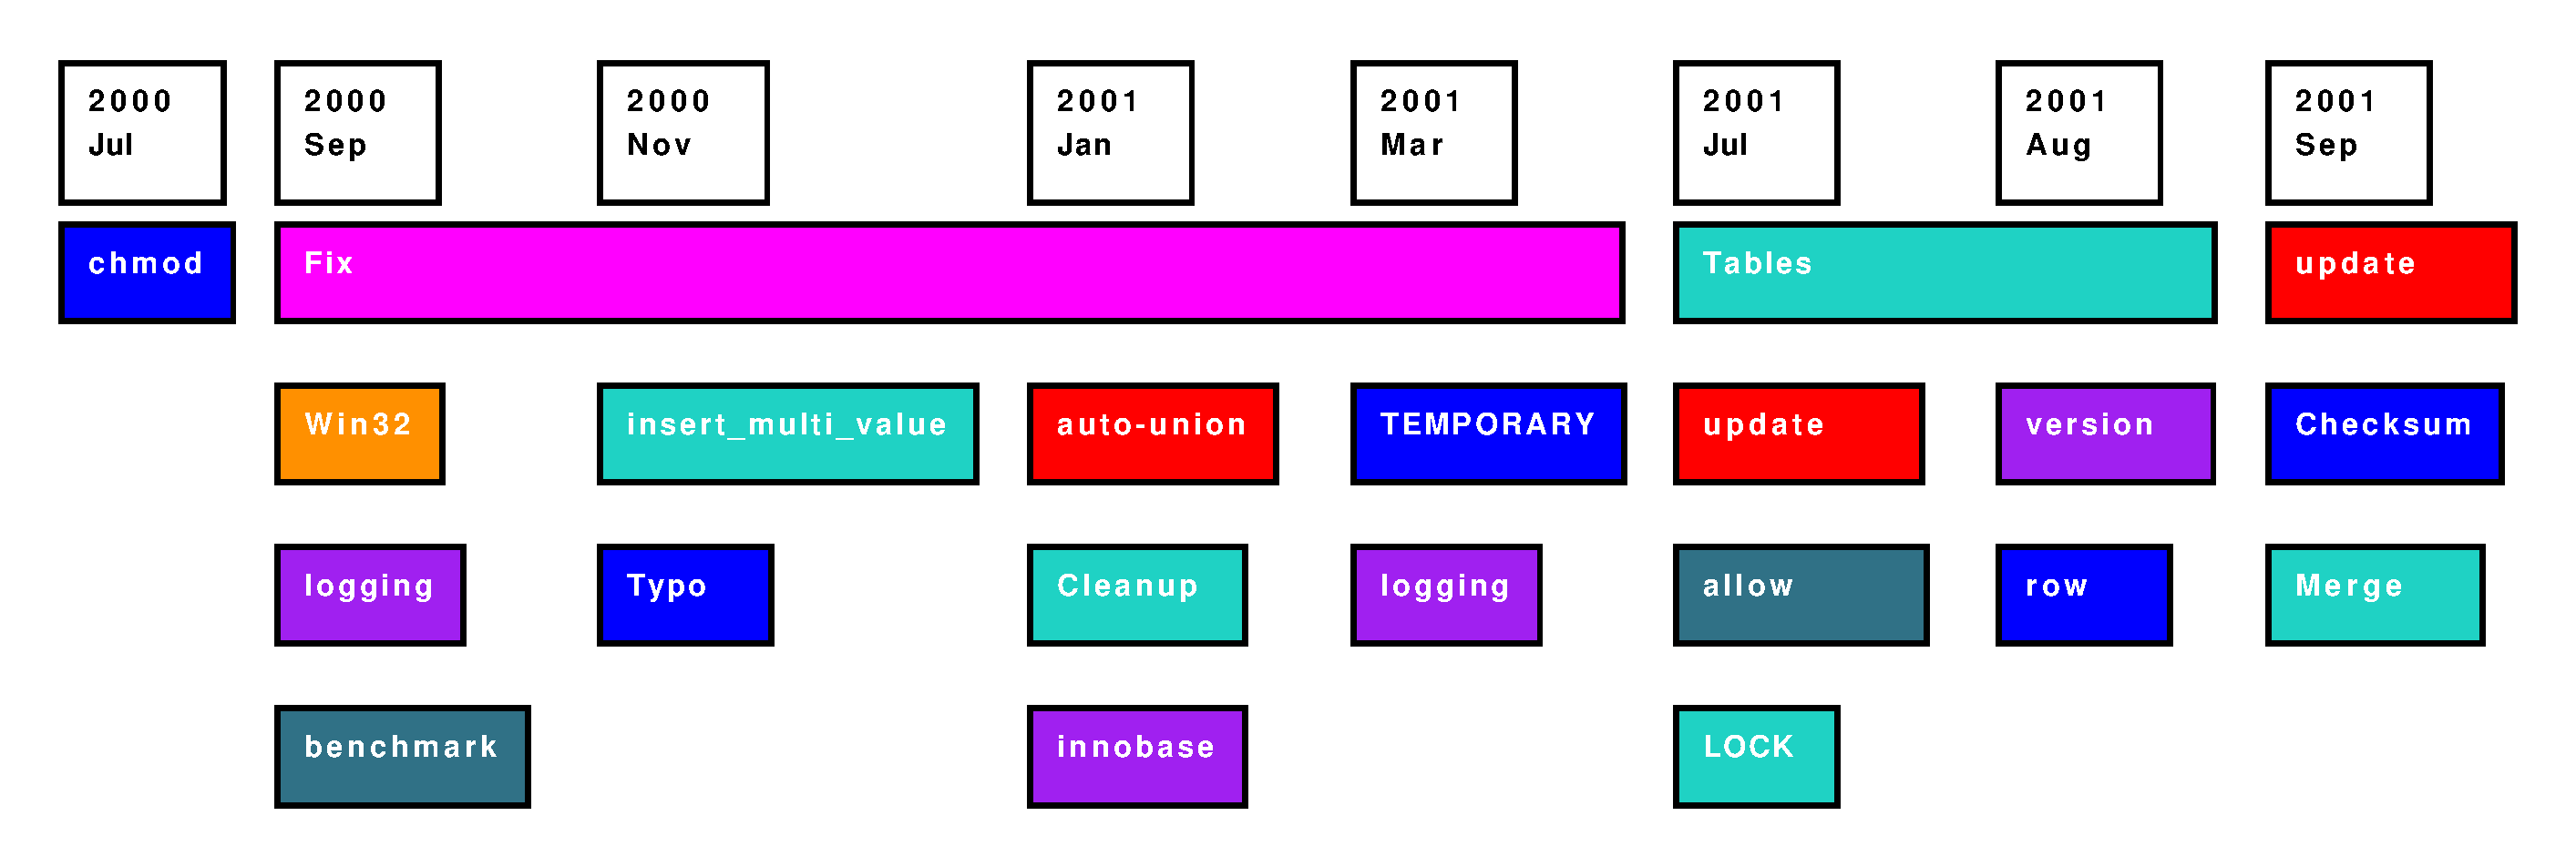
\includegraphics[width=0.9\textwidth]{lda}
  \caption{Example of topics extracted from MySQL 3.23. This is the
    kind of plot we eventually want to illustrate: named topics and
    topic trends. The horizontal axis is time by month examined. The
    vertical axis is used to stack topics that occur at the same
    time. Longer topics are topics which recur in adjacent
    windows. Colors are arbitrary.}
  \label{fig:lda}
\end{figure*}


\shrinkit
\Section{Methodology}
\shrinkit


\begin{figure*}[t]
  \centering
  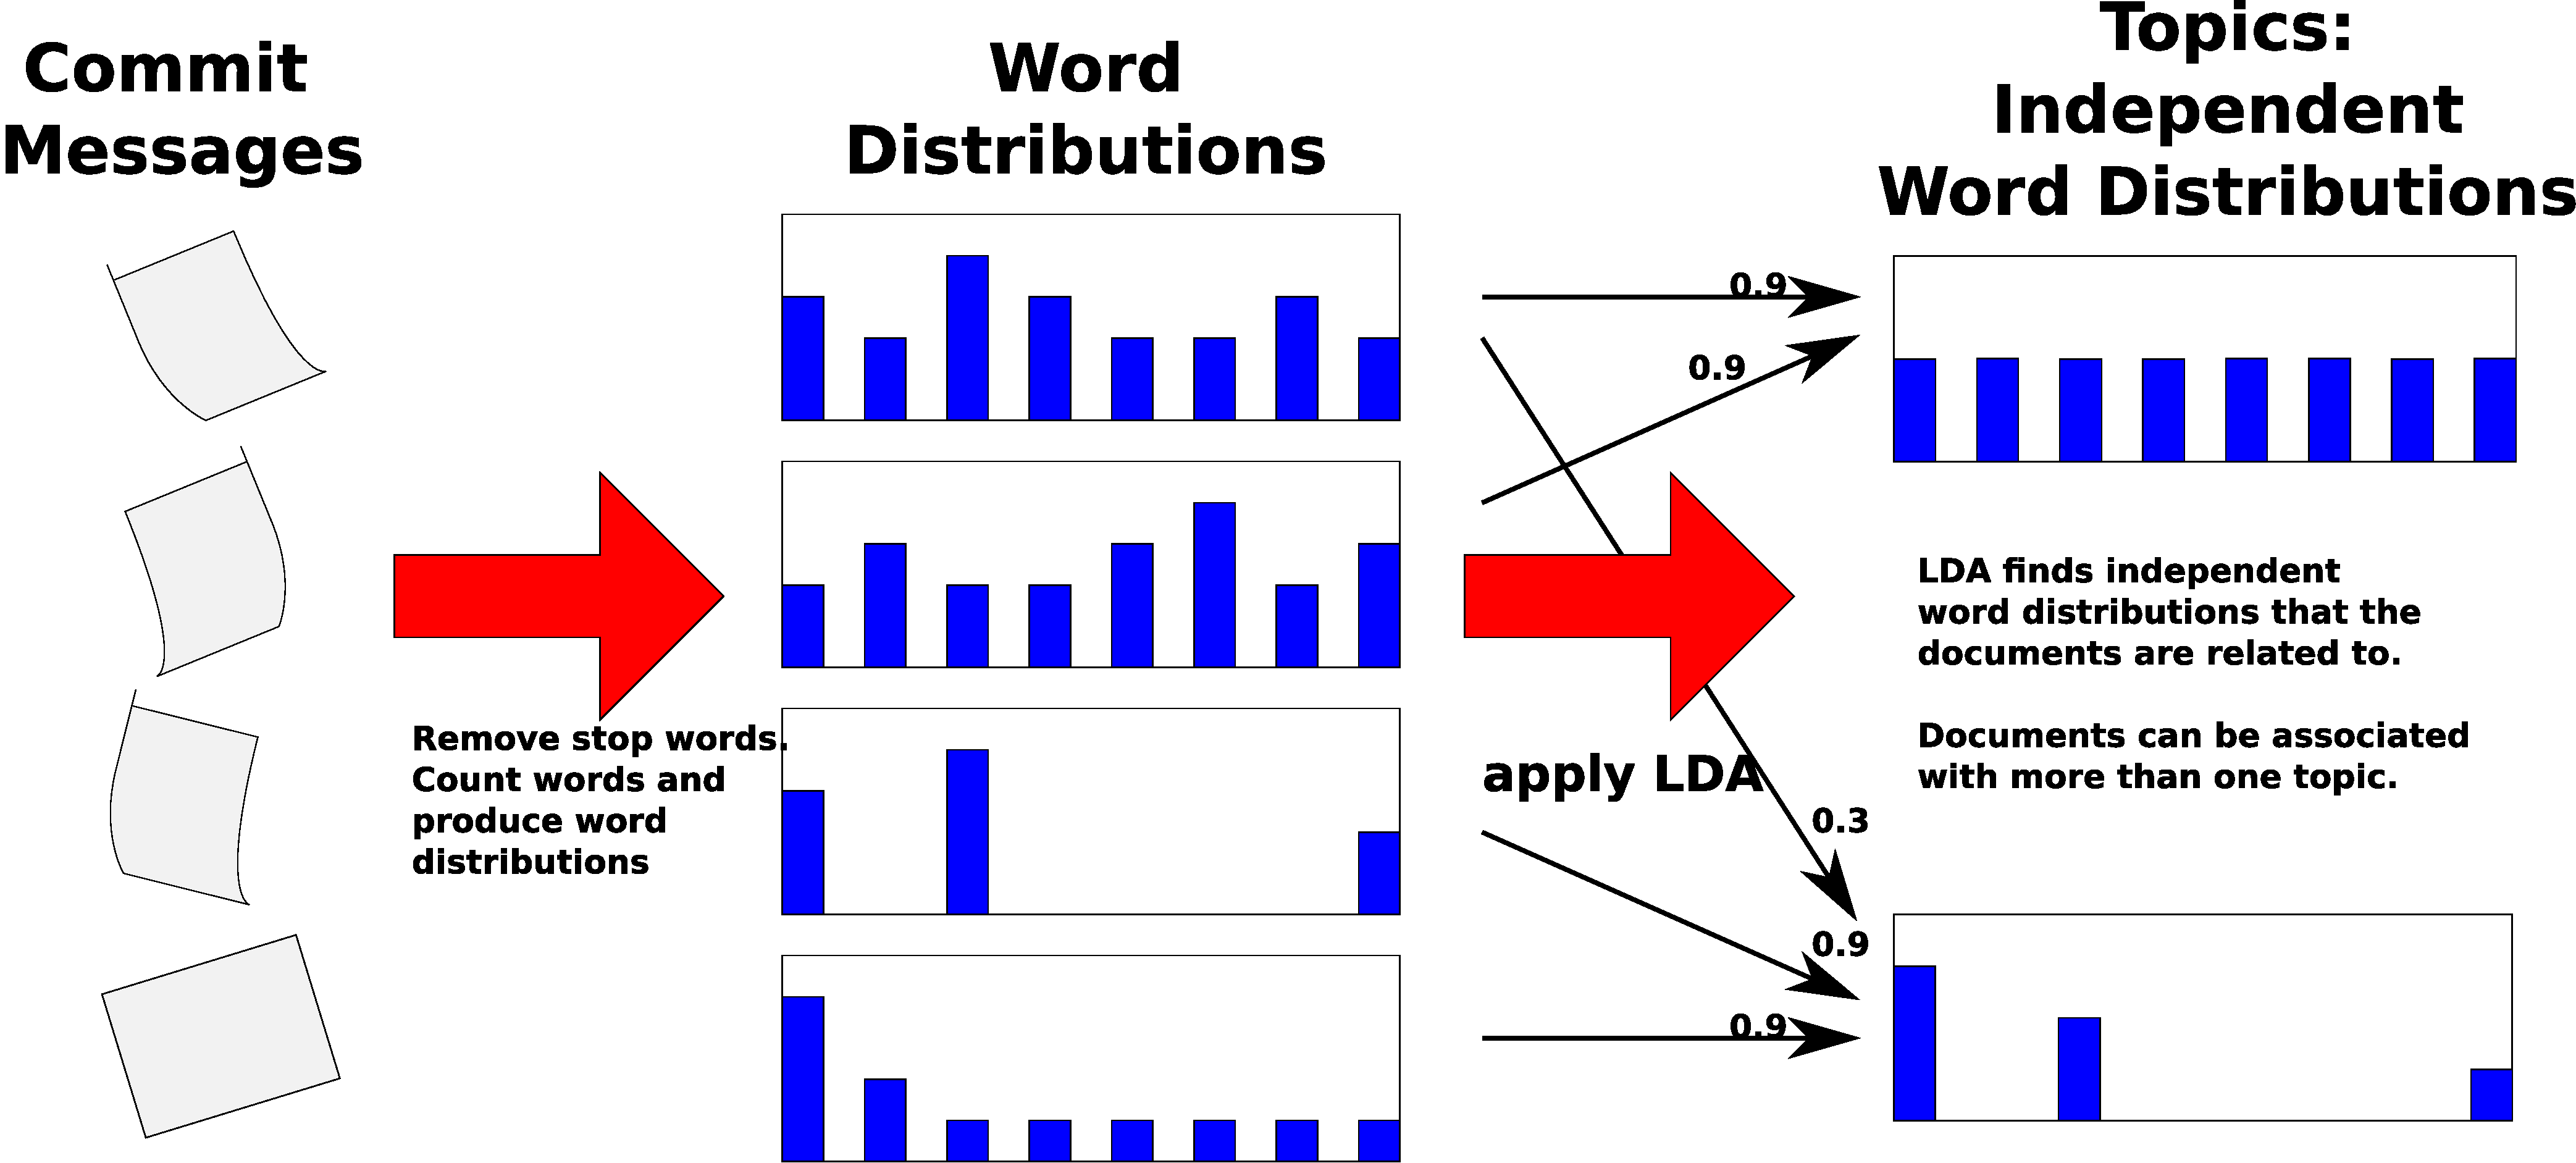
\includegraphics[width=0.9\textwidth]{commit-to-topics} 
  \caption{How commits are analyzed and aggregated into topics and trends. Commits are first extracted, then abstracted into word counts or word distributions. These word distributions are then given to topic analysis tool like LDA. LDA finds independent word distributions (topics) that these documents are related to \hlb{ (the numbers indicate similarity between documents and topics)}.}
  \label{fig:commits}
\end{figure*}


%XXX Smaller?

Our methodology is to first extract the commit log comments from a
project's SCS repository. We filter out stop words and produce word
distributions from these messages. These distributions are bucketed
into windows, and then each window is subject to topic analysis and
then we analyze and visualize the results. Figure \ref{fig:commits}
depicts the general process for processing and analyzing the commit
messages.




\shrinkit
\SubSection{Extraction of  Repositories and Documents}
\shrinkit


\hla{
We mirrored the repositories and their revisions using software such
as rsync~\cite{rsync}, CVSsuck~\cite{cvssuck},
\texttt{softChange}~\cite{dmgseke2004}, and bt2csv~\cite{methodology}.
\texttt{softChange} provided a general schema for storing revisions
and grouped CVS revisions into commits. CVSsuck and rsync mirrored CVS
repositories while bt2csv mirrored web accessible BitKeeper
repositories.
}

%XXX Smaller?

The documents we are analyzing are the commit log comments, i.e. the
comments that are added when revisions to the project are committed.
For each commit log comment, we count the occurrence of each word in
the message, remove stop words, and then produce word distributions
for each message.  These distributions are then normalized by the size
of the message, each count was divided by the total number of
tokens. After all messages are processed the distributions are
extended to include all words from all of the distributions.

\shrinkit
\SubSection{Windowed Sets}
\shrinkit

Given all messages, we group the messages into windows. We could use
overlapping windows, but in this paper we use non-overlapping windows
of a set time unit because it simplifies analysis.  
One could overlap the
windows, which would increase the likelihood of trends, but for this
study we lacked the space and were more concerned if topics ever
repeated, overlapping might skew that result.
Windowing by time
allows for many levels of granularity.  We used one month as the
length of our time windows. While we could use different window
lengths for this study we think that a month is a sizable unit of
development, which is large enough to show shifts in focus, but coarse
\hla{
enough not to show too much detail. Choosing a month as the window
provided us with enough documents to analyze. 
}

\shrinkit
\SubSection{Apply Topic Analysis to each Window}
\shrinkit

Once we have our data windowed, we apply our Topic Analysis tool to
each window and extract the top $N$ topics. We used $20$ topics in our
\hla{
case studies because we experimented before and that $20$ was about
all we can handle before too many topics seemed too indistinct from
each other to differentiate.

 Our Topic Analysis tool is an implementation of LDA.
}
We could have used other similar tools like LSI, but previous work
showed more promising topic analysis results with LDA.  We note that
this step is a slow one, as executing even one instance of LDA
involves significant computation, and we perform LDA once per window.
Figure \ref{fig:commits} shows how LDA is applied to a set of
messages, and how the topics are extracted and related to the
messages.



%\SubSection{Extract Clusters}


%   6. [ ] Cluster Similarity [0/1]
\shrinkit
\SubSection{Topic Similarity}
\shrinkit
%      1. [ ] need the tool
%             grab from the cluster analysis
%   7. [ ] Continuous Cluster Analysis


Once we have our topics extracted for each window, we analyze them and
look for topics that recur across windows.  We then cluster these
topics into trends by comparing them to each other using topic similarity.

Our input for topic similarity is the top 10 most common words of each
topic.  Each topic is compared to each other topic in the system,
given a certain threshold of top 10 word similarity, such as 8 out of
\hla{
top 10 matching words.  10 words were chosen because often people care
about top 10 comparison and it allowed for some common words to exist
but not cause topics to match so closely.  We then apply the
transitive closure on similar topics to this topic similarity matrix;
this is similar to modelling topics as nodes and similarity as arcs,
then fill flooding along the similarity arcs until we have partitioned
the topics into clusters of similar topics. Figure \ref{fig:closure}
illustrates clustering of topics by topic similarity. These clusters
of topics are called trends. 
Trends are interesting because they that topic during development has occurred over more than one period.
}

This technique has weaknesses in that nodes that are a few neighbors
away in similarity might not share any similar words.  We use this
measure because we want to be able to color or highlight topics that
are related to each other and track them throughout time.

Once we have determined our similarity clusters we are ready analyze
and to plot the topics.

\begin{comment}
Topic Clustering
 · Need to track continuous topics across
 · Similarity between topics
 · Clusters of the transitive closure of topics with X%
   similarity
    ­ Fill flood along similarity, make subsets of
      everyone who X% similar to any of their neighbors,
      make that a cluster
\end{comment}

\begin{figure}[t]
  \centering
  \includegraphics[width=0.45\textwidth]{transitiveclosure}
  \caption{Topic similarity demonstrated by clustering topics by the transitive closure (connectedness)
    of topic similarity. Nodes are topics and
    arcs imply similarity. Similarity could be a measure such as
    topics share 8 out of 10 top ten words.}
\label{fig:closure}
\end{figure}


\begin{figure*}
  \centering
%  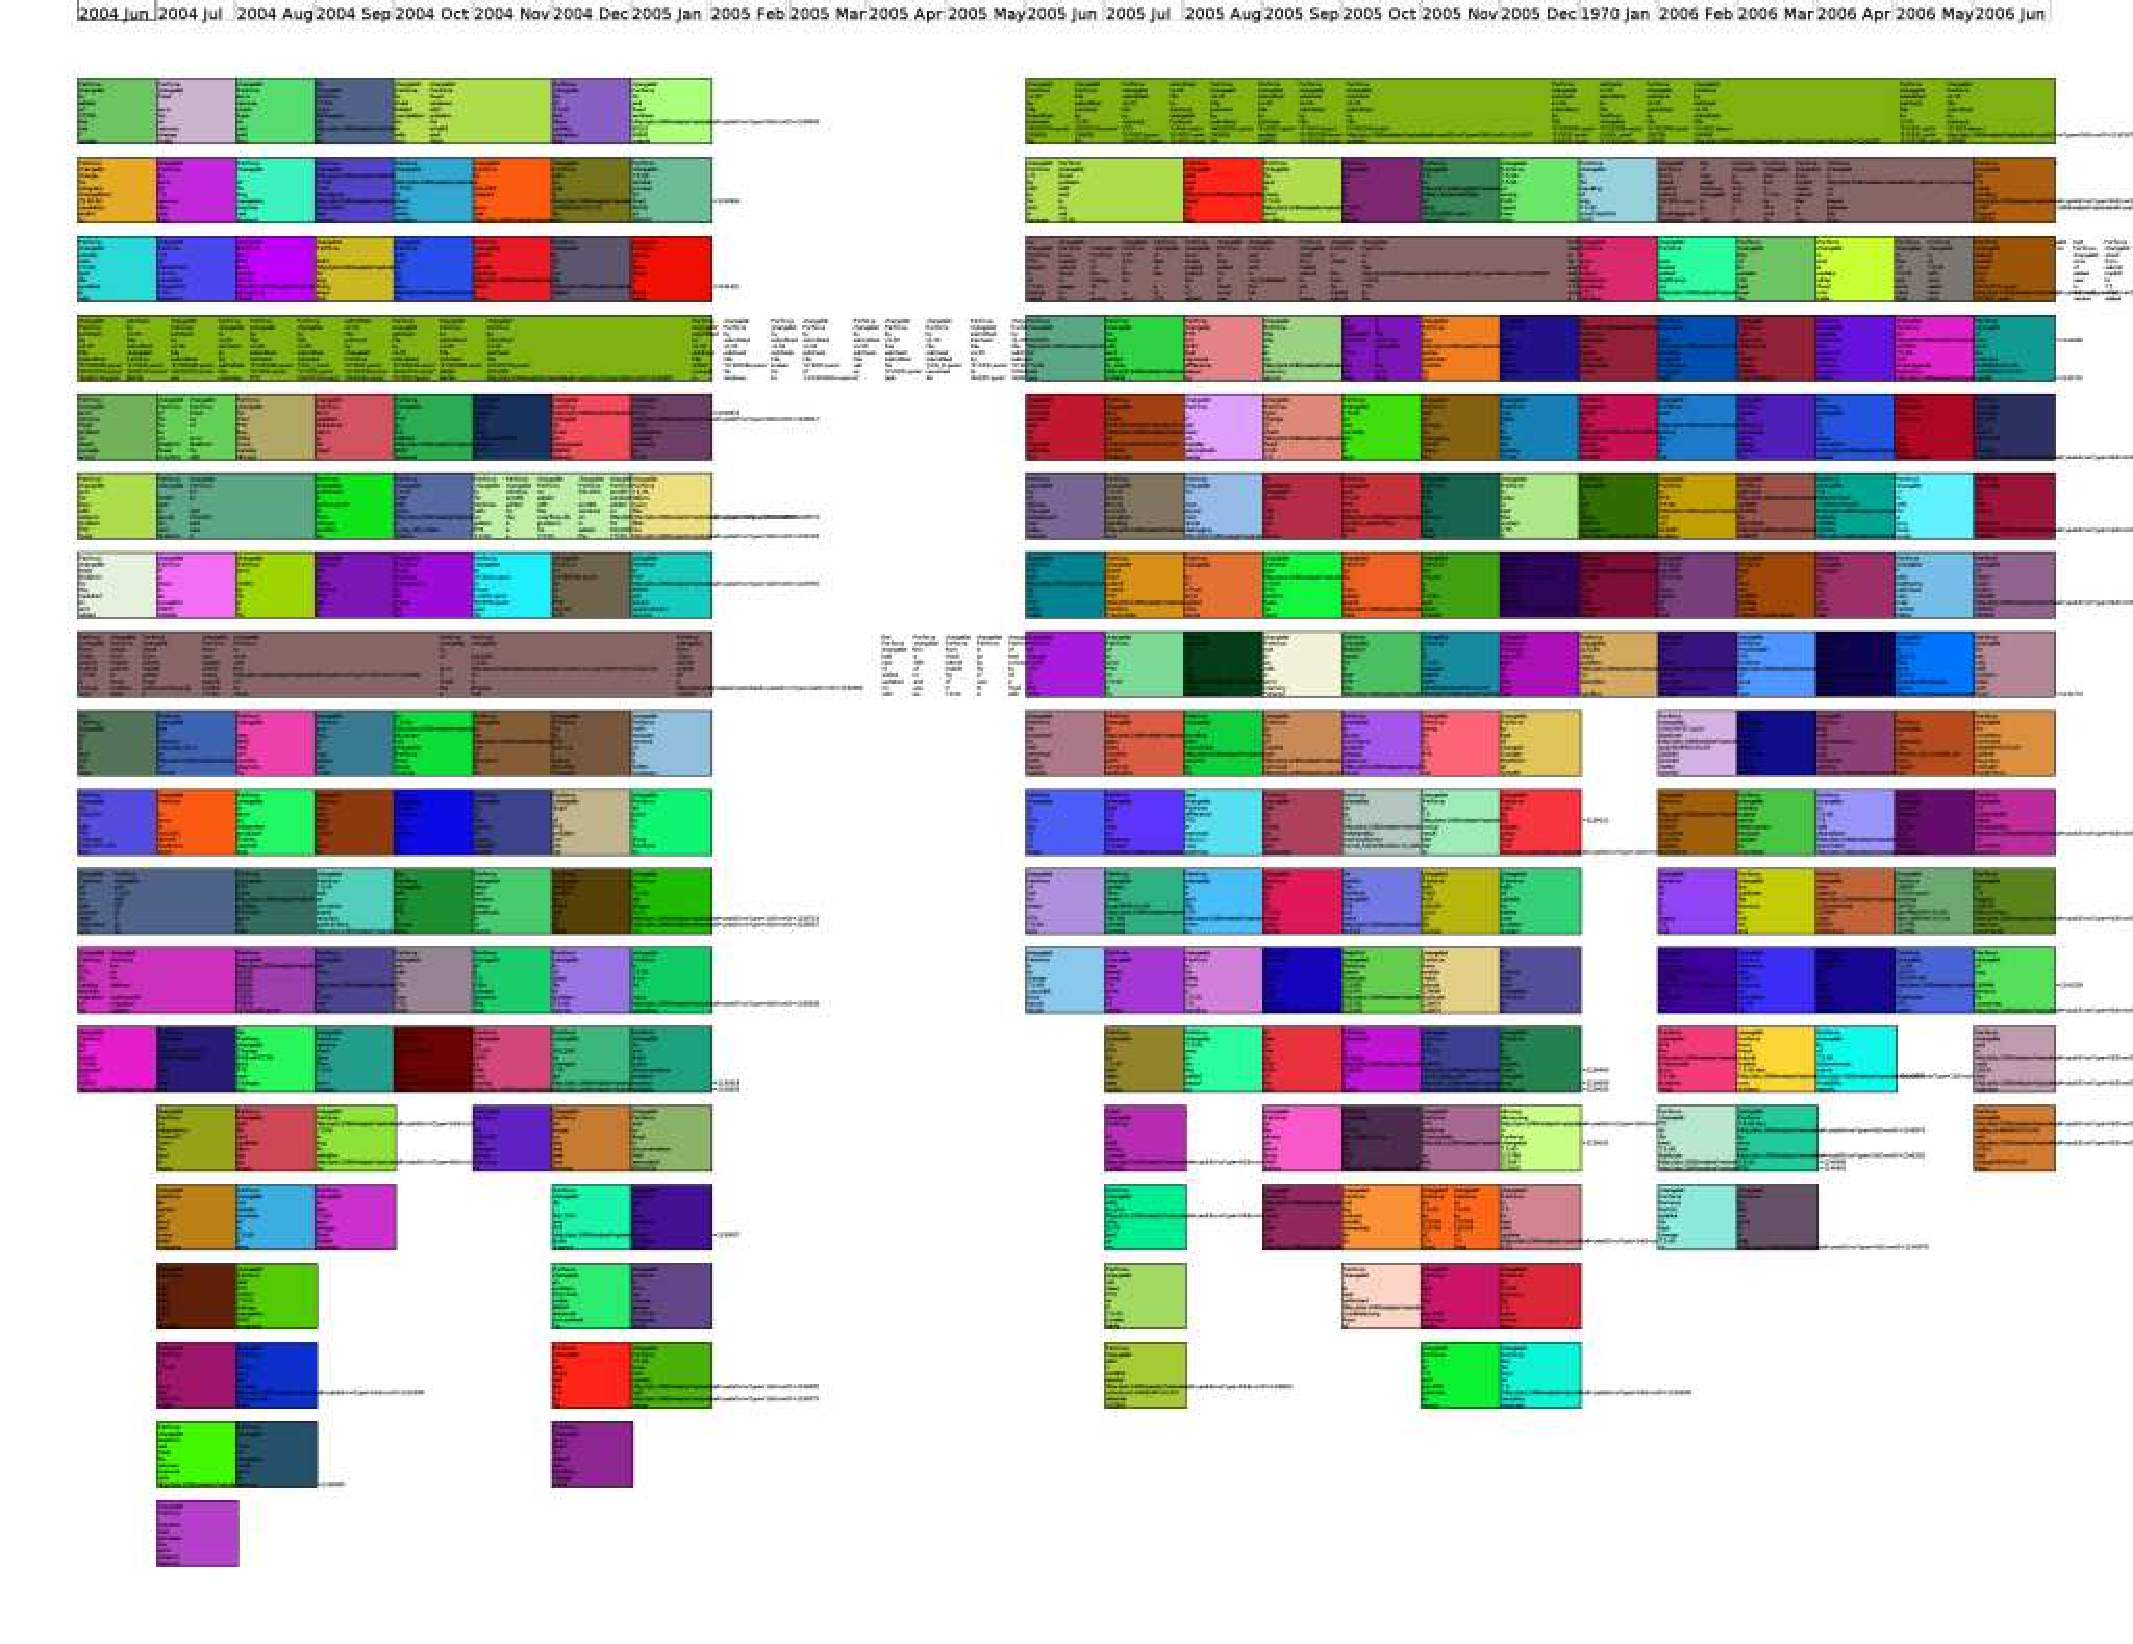
\includegraphics[width=1.0\textwidth]{fixed-time-smear-plot-scaled}
  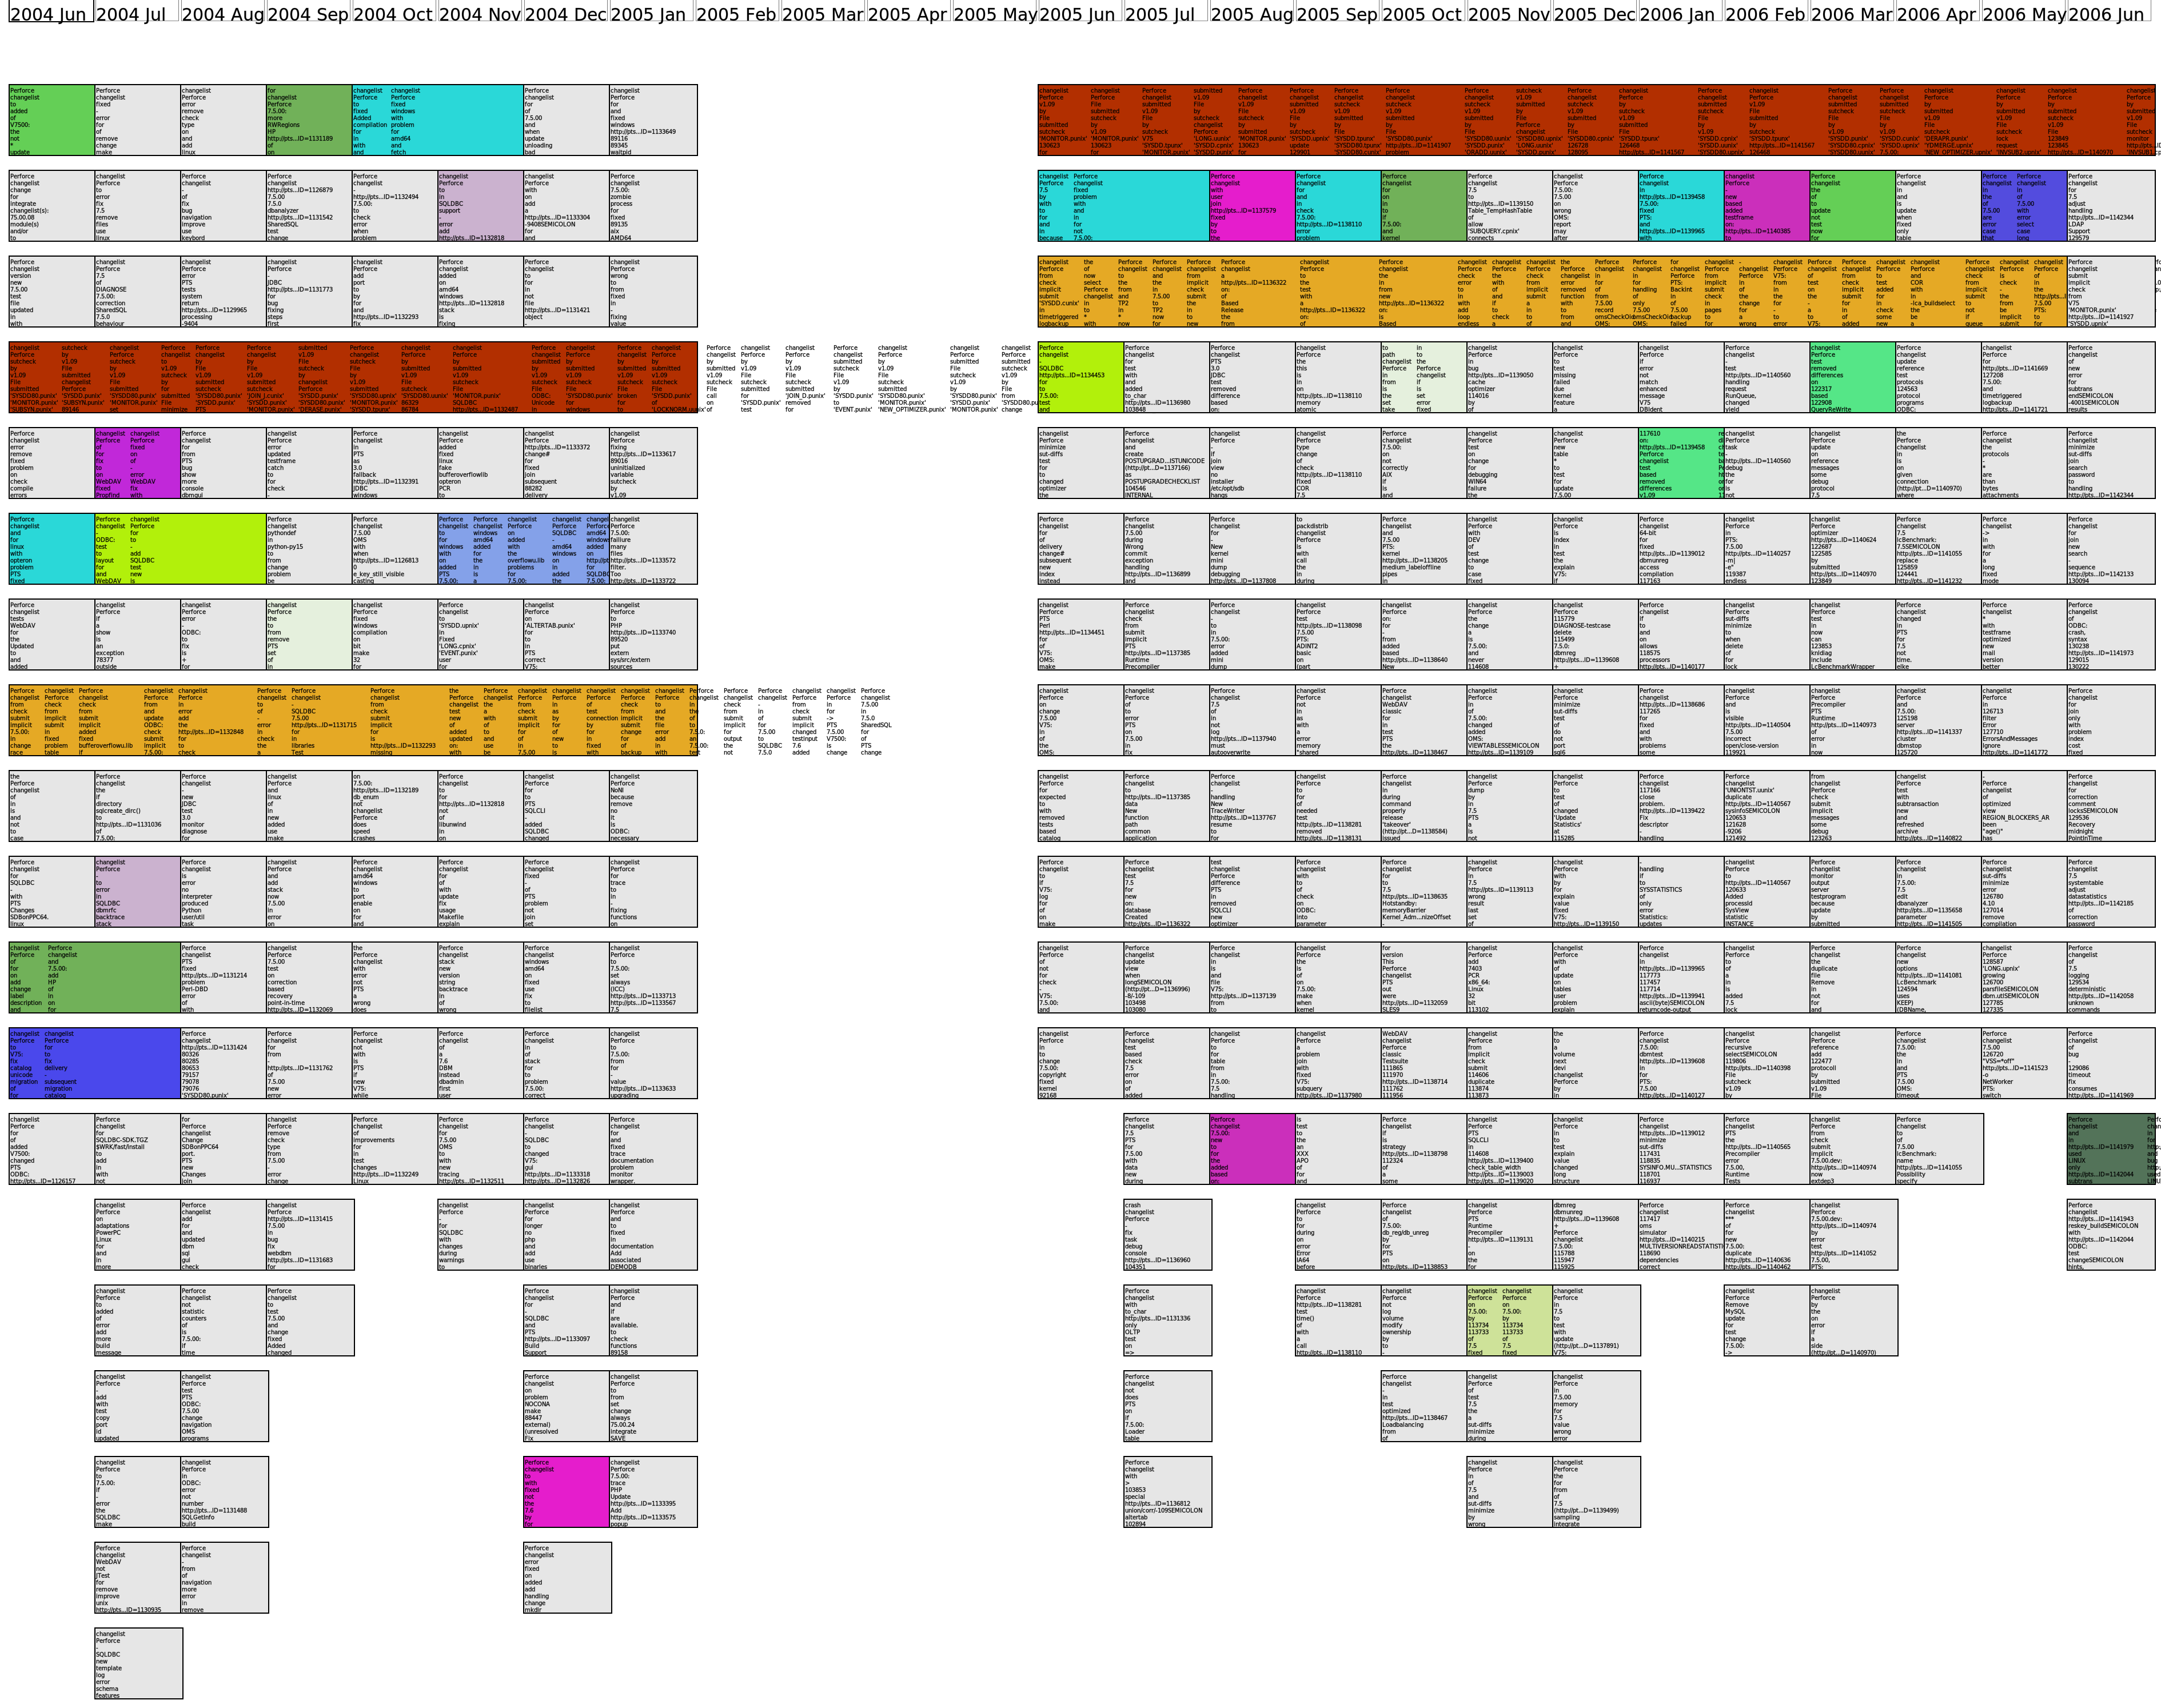
\includegraphics[width=1.0\textwidth]{time-smear-plot}%fixed-time-smear-plot-scaled}
  \caption{Compact-trend-view shows topics per month for MaxDB
    7.500. The x-axis is time in months, the Y axis is used to stack
    topics occurring at the same time. Trends that are continuous are
    plotted as continuous blocks. The top 10 words in the topics are
    joined and embedded in box representing the topics. No stop words were removed. The gap in the
    middle is a period where no development took place (see Section \ref{sec:maxdb}).}
  \label{fig:topicsmear}
\end{figure*}



\shrinkit
\SubSection{Visualization}
\shrinkit
%       1. [ ] need the visualizer
\hlb{ Visualization is an integral part of our topics analysis which
  allows us to quickly explore the topics and trends of a project.
  Visualization provides us with a framework that allows us to
  visually answer many questions about: the spread of topics, how many
  topics were independent per period, what the repeating trends were,
  if the trends dominated or did local topics dominate, how continuous
  trends were, and what the topic text in topic, trend, or period was.
  Since we have multiple questions to answer we have multiple
  visualization, described within this section, that help answer
  different questions.  }

We have devised several techniques for visualizing these topics and
trends.  For all of these techniques if we find trends that have
continuous segments, then we plot those segments as joined
horizontally across time. One technique is the \emph{compact-trend-view},
shown in Figure \ref{fig:topicsmear} and Figure \ref{fig:zoomedsmear},
that displays trends as they occur on the time-based x-axis
(placement along the y-axis is arbitrary).  Another technique is
the \emph{trend-time-line}, shown in Figure \ref{fig:trendtimeline},
each trend gets it own distinct y-value, while the x-axis is time;
these topics are then each plotted on their own line across time as
they occur. Our final technique is the \emph{trend-histogram}, shown in Figure
\ref{fig:histogram} where we plot each trend on its own line but stack
\hla{
up the segments of the trend, much like a histogram. Each topic has its top 10 words 
listed in descending order of frequency from top to bottom, this text is embedded inside the topic's box.
A trend has all of its topic text embedded side by side within the same trend box.
}

\hlb{ The \emph{compact-trend-view} (Figure \ref{fig:topicsmear})
  attempts to show all topics and trends at once across time in a
  compact view that could fit on one page. It tries to give a compact
  summary of the topics and trends across time.  } The
\emph{compact-trend-view} (Figure \ref{fig:topicsmear}) tries to sink
the larger trends to the bottom.  Once the larger trends are stacked
we fill in the gaps with the smaller trends in the same window, and
then stack the smaller trends on top.  Although there is a chance that
gaps will be left due to non-optimal stacking, in practice there are
lot of small trends (90\% of all trends contain 1 topic) that fill in
these gaps quickly.  Different instances of the same trend share the
same color; apart from that, the color of trends is randomly chosen
and color similarity is not meaningful.  The compact-trend-view is
convenient because it shows all of the topic information, as shown by
the zoomed-in view of MaxDB 7.500's compact-trend-view in Figure
\ref{fig:zoomedsmear}. The \emph{compact-trend-view} makes repeating
continuous trends easy to pick out, although discontinuous trends are
harder to spot, and provides a general summary of the topics within a project.

\hlb{
The \emph{trend-time-line} (Figure \ref{fig:trendtimeline})
attempts to show a summary of trends separated from single topics. This view shows how a trend persists across time, which aids time-wise analysis of trends.
}
The \emph{trend-time-line} displays repeating trends more clearly by
dedicating a horizontal line for trend segments belonging to one
trend. Therefore if a trend contains discontinuous segments then
the segments appear on the same line.  However, the least common
trends need to be pruned away or the view will be very long. 
Thus the \emph{trend-time-line} view is used to analyze trends across time.

\hlb{ The \emph{trend-histogram} (Figure \ref{fig:histogram}) attempts
  to show a count of how often a trend reoccurs and how many topics
  are related to a trend. It is meant to show the distribution of
  trends by their size in topics and time-span.  } The
\emph{trend-histogram} superficially resembles the trend-time-line.
However, in this view the trends are plotted together by stacking to
the left of their row, thus time information is lost.  The trends are
ordered by the number of topics in the trend.  The trend-histogram
shows the count of instances of a trend and thus indicates which
trends occur the most. Due to the large number of topics
(approximately $N$ topics multiplied by $M$ periods), given the
allotted space, it is often best to crop off the trends with only one
topic ($1\%$ to $10\%$ of the total topics), otherwise the tail is
long. \hlb{ The \emph{trend-histogram} summarizes the distribution of
trends ordered by size. }

\hlb{ All of these visualization combine to enable an analysis of
  trends and topics. Some views like the \emph{compact-trend-view}
  enable an analysis of local topics while the \emph{trend-histogram}
  and \emph{trend-time-line} focus more on trends. We used these
  visualizations to analyze the database systems that we discuss in
  the following results section.  }

\begin{figure}[t]
  \centering
  \includegraphics[width=0.45\textwidth]{fixed-time-smear-plot-cropped}
  \caption{A zoomed-in slice of compact-trend-view of topics per month of MaxDB 7.500. The topic text is visible in each topic box. Trends are plotted across time continuously.}
  \label{fig:zoomedsmear}
\end{figure}


\begin{figure}
  \centering
  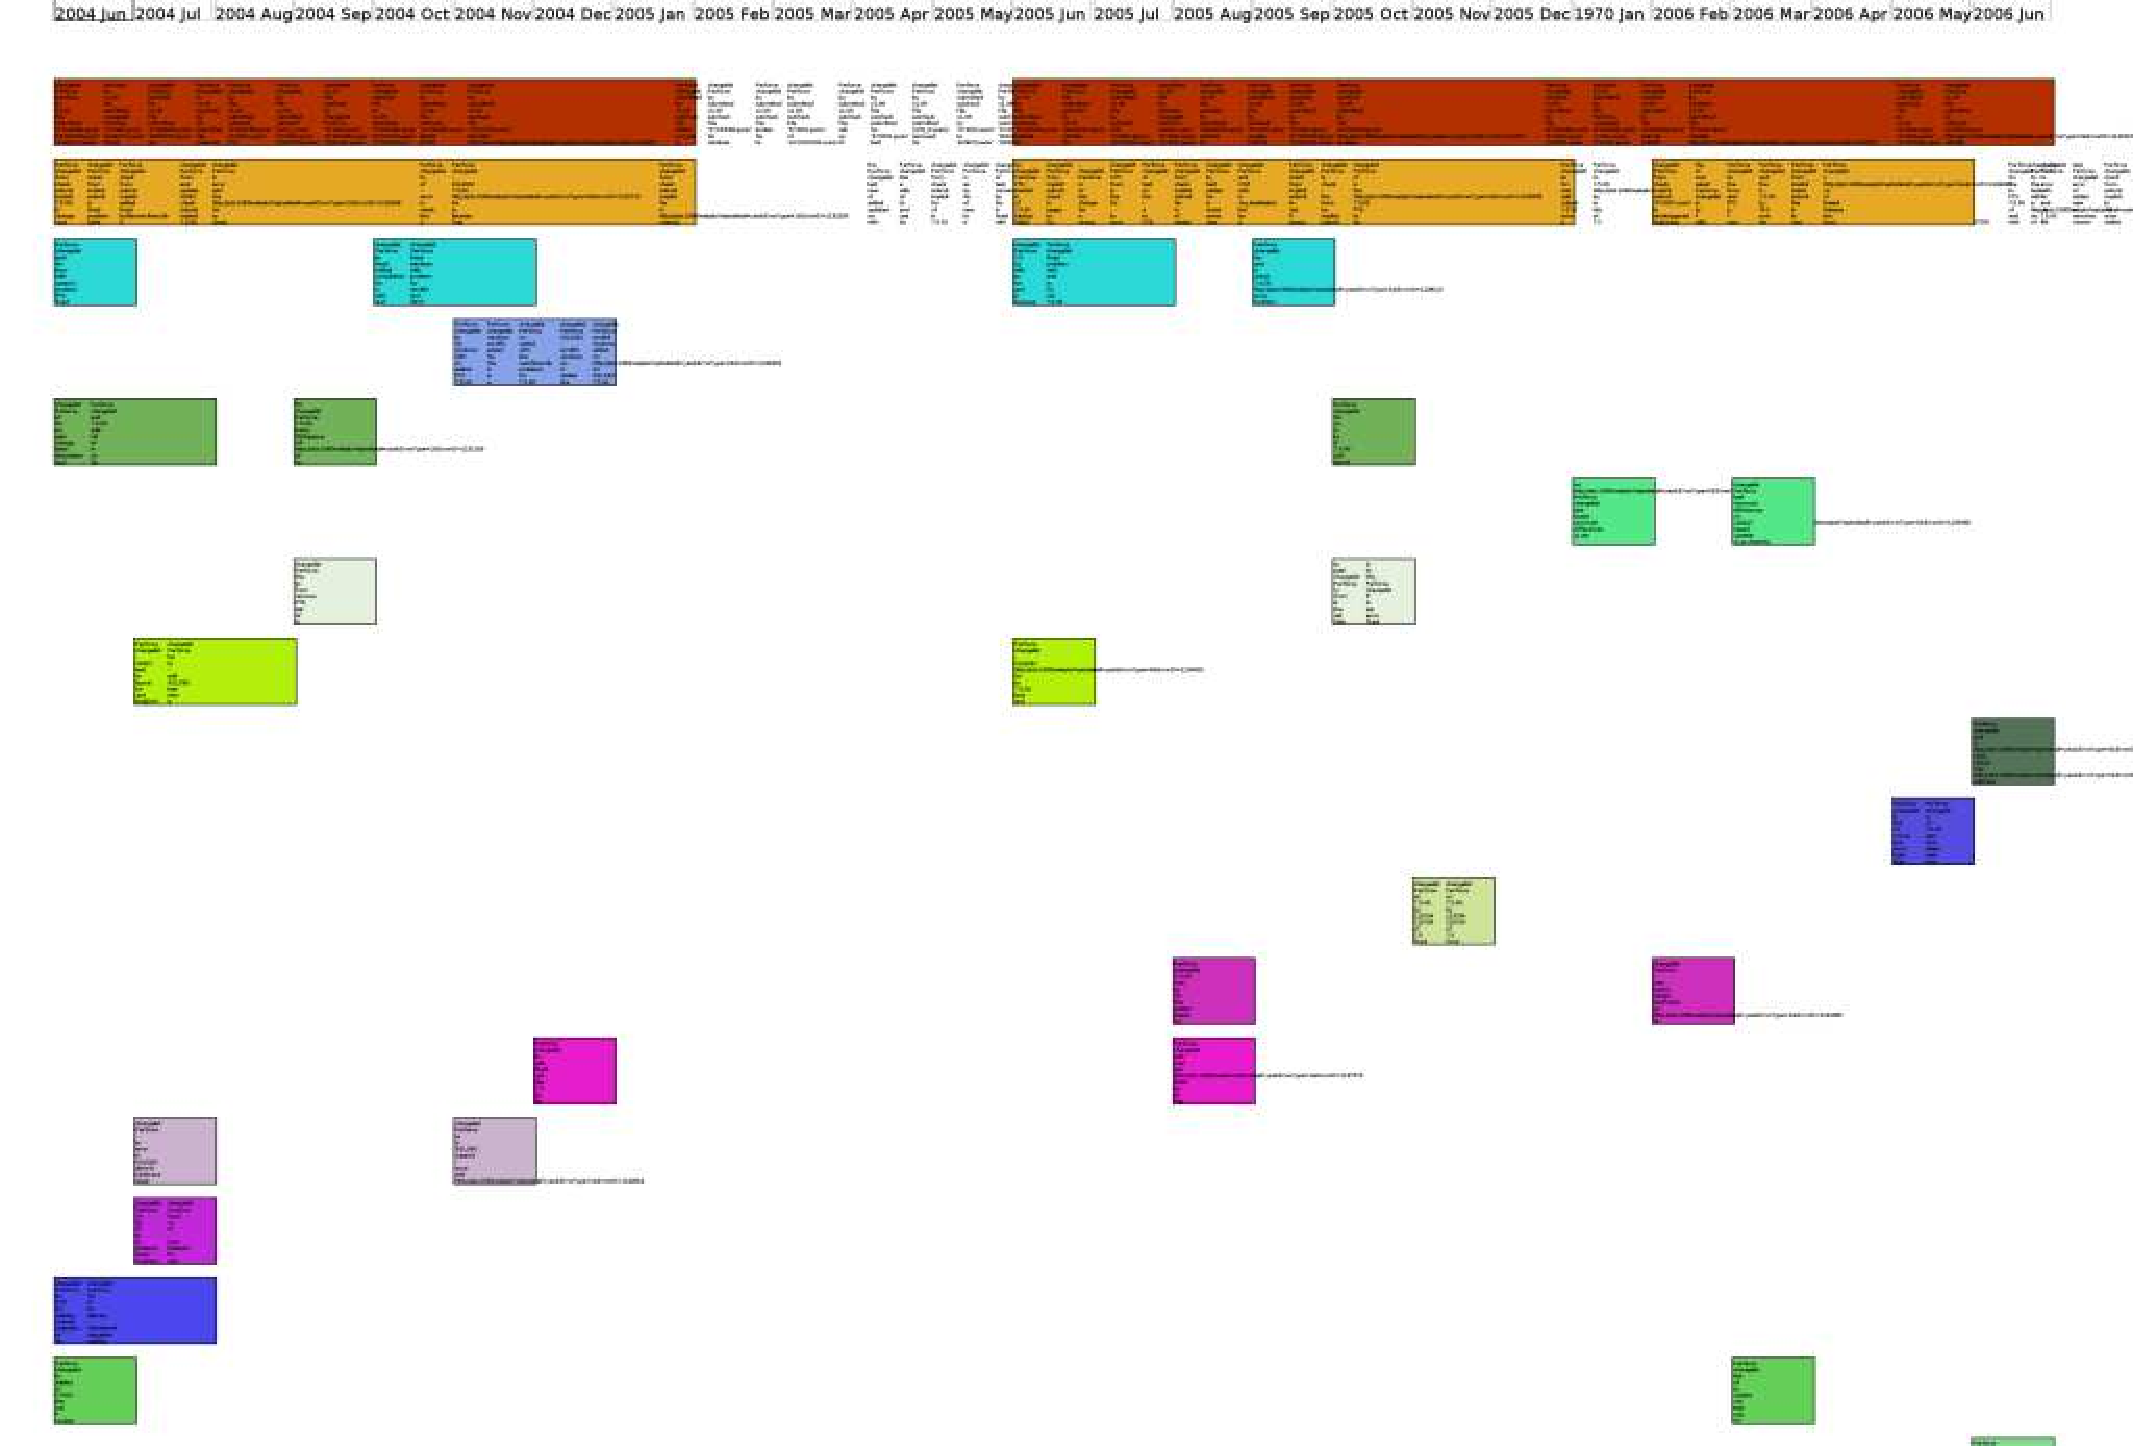
\includegraphics[width=0.45\textwidth]{class-smear-plot-crop-scaled}
  \caption{Trend-time-line: Trends plotted per month of MaxDB 7.500. Time in months are plotted along the x-axis, each row on the y-axis is associated with a trend ranked by size in descending order}         
  \label{fig:trendtimeline}
\end{figure}


\begin{figure}
  \centering
  \includegraphics[width=0.45\textwidth]{histogram-cropped-scaled}
  \caption{The top part of a trend-histogram of MaxDB 7.500, ordered
    by topic occurrence. X-axis determines the number of continuous
    months of a trend. Trends are ranked by the number of topics that
    a trend contains in descending order.}
  \label{fig:histogram}
\end{figure}



\shrinkit
\Section{Results}
\shrinkit

We applied our methodology to multiple database systems that we
extracted.  To analyze these extracted repositories we used:
Hiraldo-Grok, an OCaml-based variant of the Grok query language;
Gnuplot, a graph plotting package; lda-c, a LDA package implemented by
Blei et al.~\cite{944937}; and our trend plotter, implemented in
Haskell.

We applied our tools and visualizations to the repositories of these
\hla{
open source database systems: PostgreSQL, MaxDB and Firebird. The
total number of commits analyzed was over $66 000$.
}

%\SubSection{MySQL}
%XXX DO MYSQL?
\shrinkit
\SubSection{PostgreSQL}
\shrinkit
%   3.   mysql


When we examined PostgreSQL's history from 1996 to 2004, which includes
over $20 000$ commits. We did not find many trends with two or more
topics, using a similarity of $7/10$. $7/10$ was chosen because it
preserve independent topics but seemed to be a threshold
value where more serious trends started to appear.

Those trends that we did find
were not very large, lasting only 3 months at most. The first and second
largest trends directly referenced two external developers:
Dal Zotto, Dan McGuirk. The fifth largest trend related to work by
PostgreSQL developer D'Arcy. Other topics of the larger trends were
changes to the ``to do'' list, and time string formating topics
relating to time-zones.

If we kept the stop words we found that the large trend consisted
mostly of stop words and non-stop words such as \emph{patch},
\emph{fix}, \emph{update}.  By decreasing the similarity constraint to
$1/2$ the largest most common trend, which stretched across
the entire development, contained these same words (\emph{patch},
\emph{fix}, \emph{update}). The second largest trend mentions Dal
Zotto, while the third largest trend mentions the \texttt{[PATCHES]}
mailing-list and the names of some patch contributors.  Other repeating
topics refer to portability with Win32, Central Europe Time (CEST)
from email headers, issues with ALTER TABLE and CVS branch merging
(CVS does not record merges explicitly).


\shrinkit
\SubSection{Firebird}
\shrinkit
%   5.   what's that other db?


\hla{
We tracked Firebird from August 2000 to January 2006, we extracted comments from $38 000$ commits. We found that with a
}
similarity of $7/10$ Firebird had far more continuous and
recurring trends than PostgreSQL.  The first large trend was discontinuous
across time but explicitly references one author \texttt{carlosga05}
and words like \emph{added}, \emph{fixed} and \emph{updated}.

The second largest trend was during the month of March 2001. It was
related to incremental building and the porting of developer
Konstantin's Solaris port of the Firebird build files. The third
largest trend was about JDBC, which is how Firebird and Java
communicate.  Other trends included topics regarding AIX PPC
compilation, updating the build process, internationalization and
UTF8, Darwin build support and bug fixing.

Topics that were not trends but appeared to be interesting were mostly
external bug fixes submitted to the project.  In these cases, the
developers would express gratitude in their commit log comments, such
as ``Thanks, Bill Lam''.  Other easily discernible topics included
tokens and phrases such as: \emph{compiler workarounds}, \emph{nightly
  updates}, \emph{packets} and \emph{MSVC++}.


\shrinkit
\SubSection{MaxDB 7.500}
\shrinkit

\label{sec:maxdb}

% Migod todo
% I think that you should enlarge this discussion of MaxDB (at the
% expense of the other systems) and make careful references to how the
% diagrams give you extra info about the evolution of the system (in
% terms of topics).

% We are trying to argue that (a) the approach is more informative that
% the naive static approach and (b) the diagrams are useful.



The plots we produced of MaxDB 7.500 were unlike those of the other
\hla{
systems, as there was a period where no development occurred and thus
there were no topics or trends whatsoever (see the gap in Figure
\ref{fig:topicsmear}). Using a topic similarity of $7/10$ we evaluated
MaxDB 7.500. MaxDB 7.500's first period was from June 2004 to January
2005, and its second period was from June 2005 to June 2006. There
were a total of $8 600$ commits analyzed.
}

The largest common trend has references to build system files like
\texttt{SYSDD.punix} and \texttt{MONITOR.punix}.  This trend is
partially displayed at the top of the zoomed in compact-trend-view
(Figure \ref{fig:zoomedsmear}) and at the top of the trend-histogram
(Figure \ref{fig:histogram}).  Other tokens mentioned are
\emph{Sutcheck v1.09} (the prefix SUT stands for Storable Unit Type),
\emph{Sutcheck} is a tool that would also automate check-ins using a Perforce SCS
tool, which was exporting check-ins to CVS.

The second largest common trend seems to be a side effect of an
automated check-in that is annotated as ``implicit check-in'' (see
the bottom of Figure \ref{fig:zoomedsmear}). These were check-ins that
were produced when importing changes from an external Perforce
repository.

The third most common trend, seen on Figure \ref{fig:trendtimeline},
seemed to include tokens related to operating system support, such as
\emph{Linux} and \emph{Windows}, as well as architecture support, \emph{AMD64} and
\emph{Opteron}. The word \emph{problem} was common among all of these
trends. This trend seemed related to the smaller fourth largest trend
that had tokens \emph{AMD64} and \emph{Windows}. This example shows that
topics can overlap but still not match via our similarity measure.


%XXX Edit
% Was reading lda.report
Bug tracker URLs dominated unique topics during some months. For
instance in the last month of MaxDB 7.500 development every topic
contained one unique Bug tracker URL. This pattern did not occur in the
previous month. We investigated the revisions and we found that
developers were referencing the bug tracker more during the last
month.  If the topics of one month were about unique bug tickets being
addressed, the global topic analysis would probably miss this, yet
these bug tickets were the focus of development for that month but not
necessarily globally relevant.

The query optimizer was a topic that recurred during MaxDB's
development. In our plots, topics that mention \emph{optimizer} occur
four times, yet in the global-trend-view (Figure
\ref{fig:statictopics}, explained in Section \ref{sec:compare}) it is not in any of the topics. A query
optimizer is an important component of an DBMS, but as we have shown
it does not appear as a topic on its own. We tried to remove words to
see if we could get an \emph{optimizer} topic. After removing stop
words and then two of the most common words, the global analysis
\hla{
finally had a topic with optimizer in its topic ten words. Our
analysis shows that optimizer was important but it had been obscured
by the global topic analysis, which used the entire history of
messages, but would have been noticed using the more local topic
analysis such as our windowed topic analysis, which used a window of
messages.
}

We noticed that commits that mentioned \emph{PHP} occurred two thirds
less frequently than commits that mentioned \emph{Perl}, but
\emph{Perl}-related topics appeared in the global static topics for
MaxDB while \emph{PHP}-related topics did not.  Our local topic
analysis mentioned \emph{PHP} in 5 different topics, yet only
mentioned \emph{Perl} in four different topics and one global
topic. Perhaps this is because there was a cluster of \emph{Perl}
mentions during one month while the \emph{PHP} mentions were more
spread out.

Just about every topic included the words \emph{Perforce} and
\emph{Changelist}, so we added them to the stop words list. As a
result, longer trends were shortened and sometimes the total number of
topics found per month were reduced.  Evaluating different similarity
thresholds showed that by removing common words one reduces the
general similarity of topics. That said, the larger topics were still
clearly apparent. Thus if more relevant stop words are added one
should tune the topic similarity parameters to handle these changes.



% UNICODE
% DEC/OSF1
% ODBC
% crash
% PHP yet Perl is mentioned is less but it part
% SQLCLI
% %V75
% SYSDD.cpnix
% backup
% select
% make
% memory
% view
% debug
% V75 is mentioned many times maxdb version guh


\shrinkit
\SubSection{Compare with topics over the entire development}
\shrinkit

\label{sec:compare}

% Migod notes This section is perhaps the most important of the
% whole paper.  You need expand it.  Maybe you should move the first
% two paras of the conclusions in here too.

% The thing that is most disappointing is that the argument is entire
% qualitative.  Can you give examples to make this sound less
% hypothetical?

% Can you add numbers in here to make the argument stronger?


% Previous work on topic analysis that employed LSI and LDA typically
% extracted a specified number of topics and then tracked their
% relationship to documents over time. This means that a single, static
% set of topics was tracked across the whole development history of a
% project, we refer to this as \emph{global topic
%   analysis}.% is topic analysis applied against the entire lifetime of a
% %project.

Previous work on topic analysis that employed LSI and LDA typically
extracted a specified number of topics from the entire development
history of a project and then tracked their relationships to documents
over time, we call this \emph{global topic analysis}.

% This means that a single, static
%set of topics was tracked across the whole development history of a
%project, we refer to this as \emph{global topic
%  analysis}.% is topic analysis applied against the entire lifetime of a
%project.

We carried out \emph{global topic analysis} on MaxDB 7.500 and
compared this against our windowed topic analysis.  To produce
Figure~\ref{fig:statictopics}, we extracted 20 topics and plotted the
number of messages per month that were related to that topic.  One
topic would often dominate the results, as shown in the third row of
Figure \ref{fig:statictopics}, while the other topics did not appear
as often.

% This technique seems useful if the 20 extracted topics are relevant
% and useful, that said one weakness of this approach is that documents
% for a topic might only occur in one time window, yet we are tracking
% messages that could be related to it over the entire lifetime of the
% project.
This approach seems reasonable if most of the extracted topics are of
broad interest during most of the development process.  However, it
may be that some topics are of strong interest but only briefly; in
such a case, a windowed topic analysis gives a much stronger
indication of the fleeting importance of such topics, and can help to
put such a topic into its proper context.

% Revisions 26+1+103+19+20+48+35+50+77+49+48+18
% Revisions 494 
% Topics 1+1+19+1+5+10+7+10+11+9+9+7
% Topics 90

If we approach the difference of global topic analysis and windowed
topic analysis via common tokens we can see that common tokens tend to
dominate both results. For MaxDB 7.500, our local topic approach
netted us topics that contained these relatively important and common
words, which did not occur in the topics produced by global topic
analysis: \emph{UNICODE}, \emph{DEC/OSF1}, \emph{ODBC}, \emph{crash},
\emph{SQLCLI}, \emph{SYSDD.cpnix}, \emph{backup}, \emph{select},
\emph{make}, \emph{memory}, \emph{view}, and finally
\emph{debug}. \emph{ODBC} is an important topic token, because it
often determines how databases communicate with software. None of
these tokens were part of the global topic analysis topics, but they
were part of 566 commits (6\% of the entire system) to MaxDB
7.500. These tokens were part of 87 out of 520 (26 months, 20 topics
per month) of our locally generated topics.

%XXX Numbers and more argument

Even with our liberal topic similarity metrics that produced both long
and short trends, we showed that there are only a few trends in a
repository that recur. Since so few trends recur and so many trends
appear only once this suggests that global topic analysis might be
ignoring locally unique topics.

The utility of global topic analysis is questionable if the value of
information decreases as it becomes older. Perhaps older trends will
dominate the topic analysis. Windowed localized topic analysis shows
what are the unique topics, yet seems to give a more nuanced view of
the timeliness of the important topics.


\begin{figure}[t]
  \centering
  %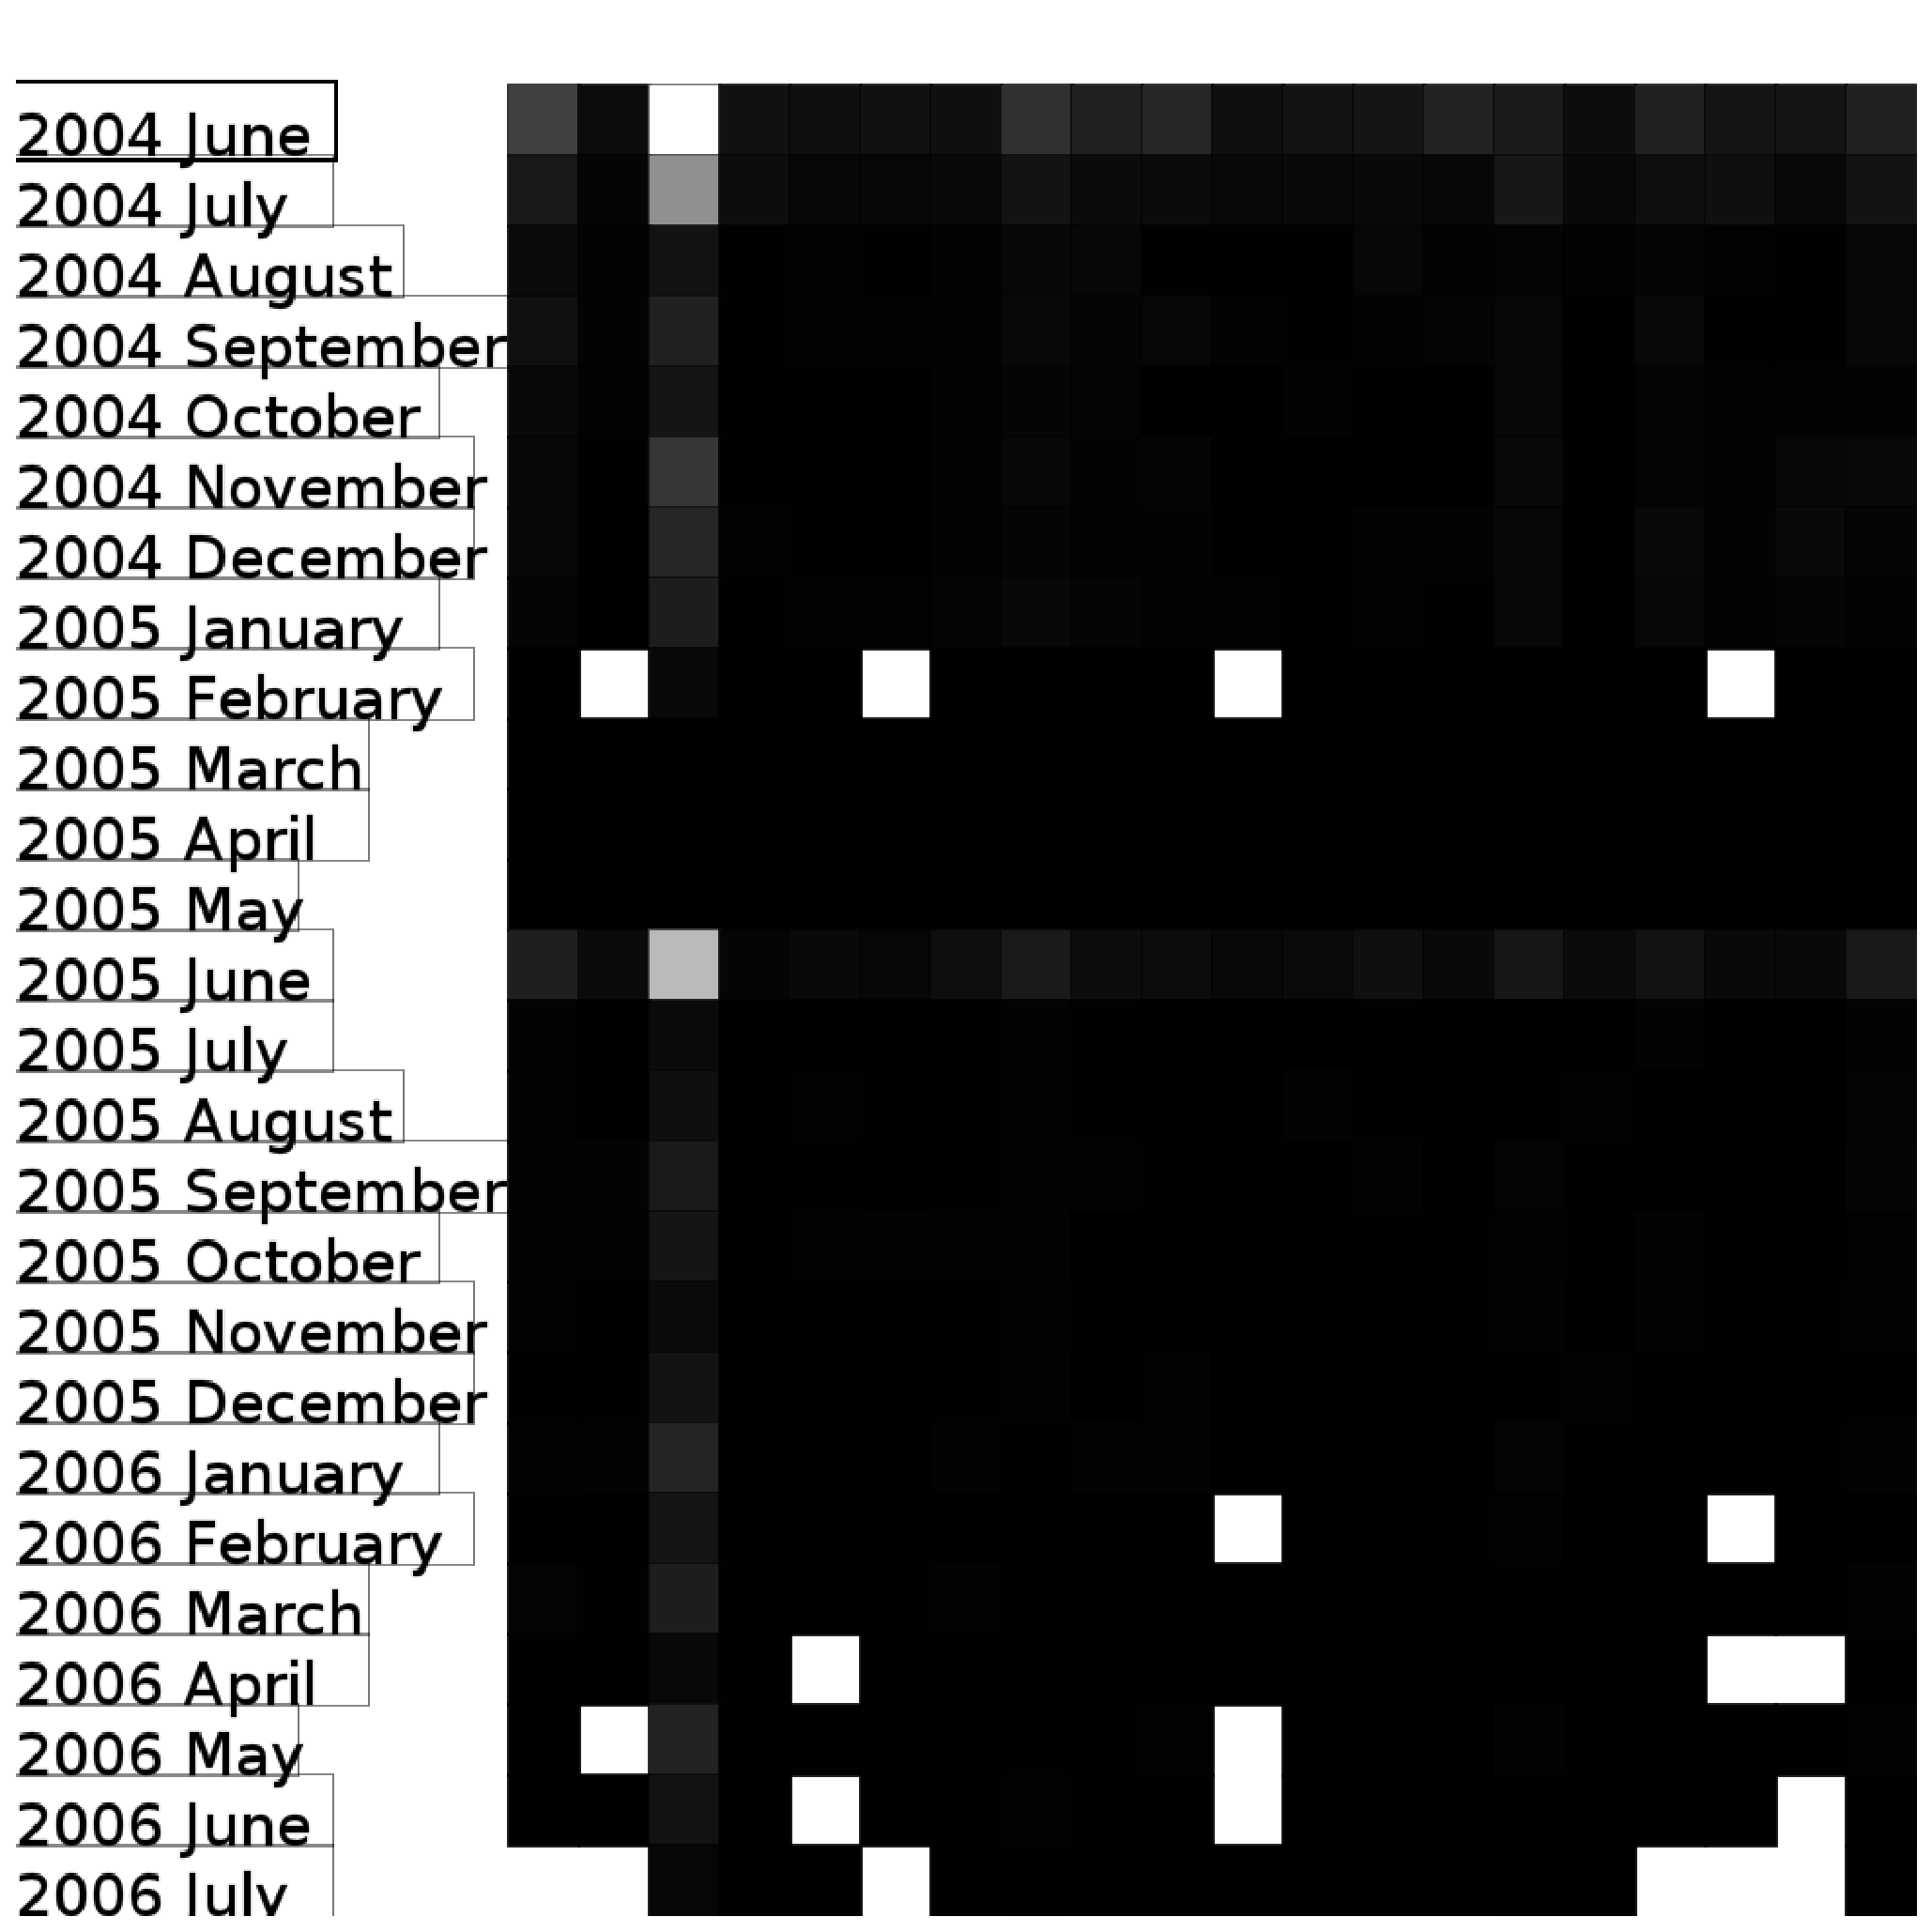
\includegraphics[width=0.45\textwidth]{maxdb7500-everything-by-month}
  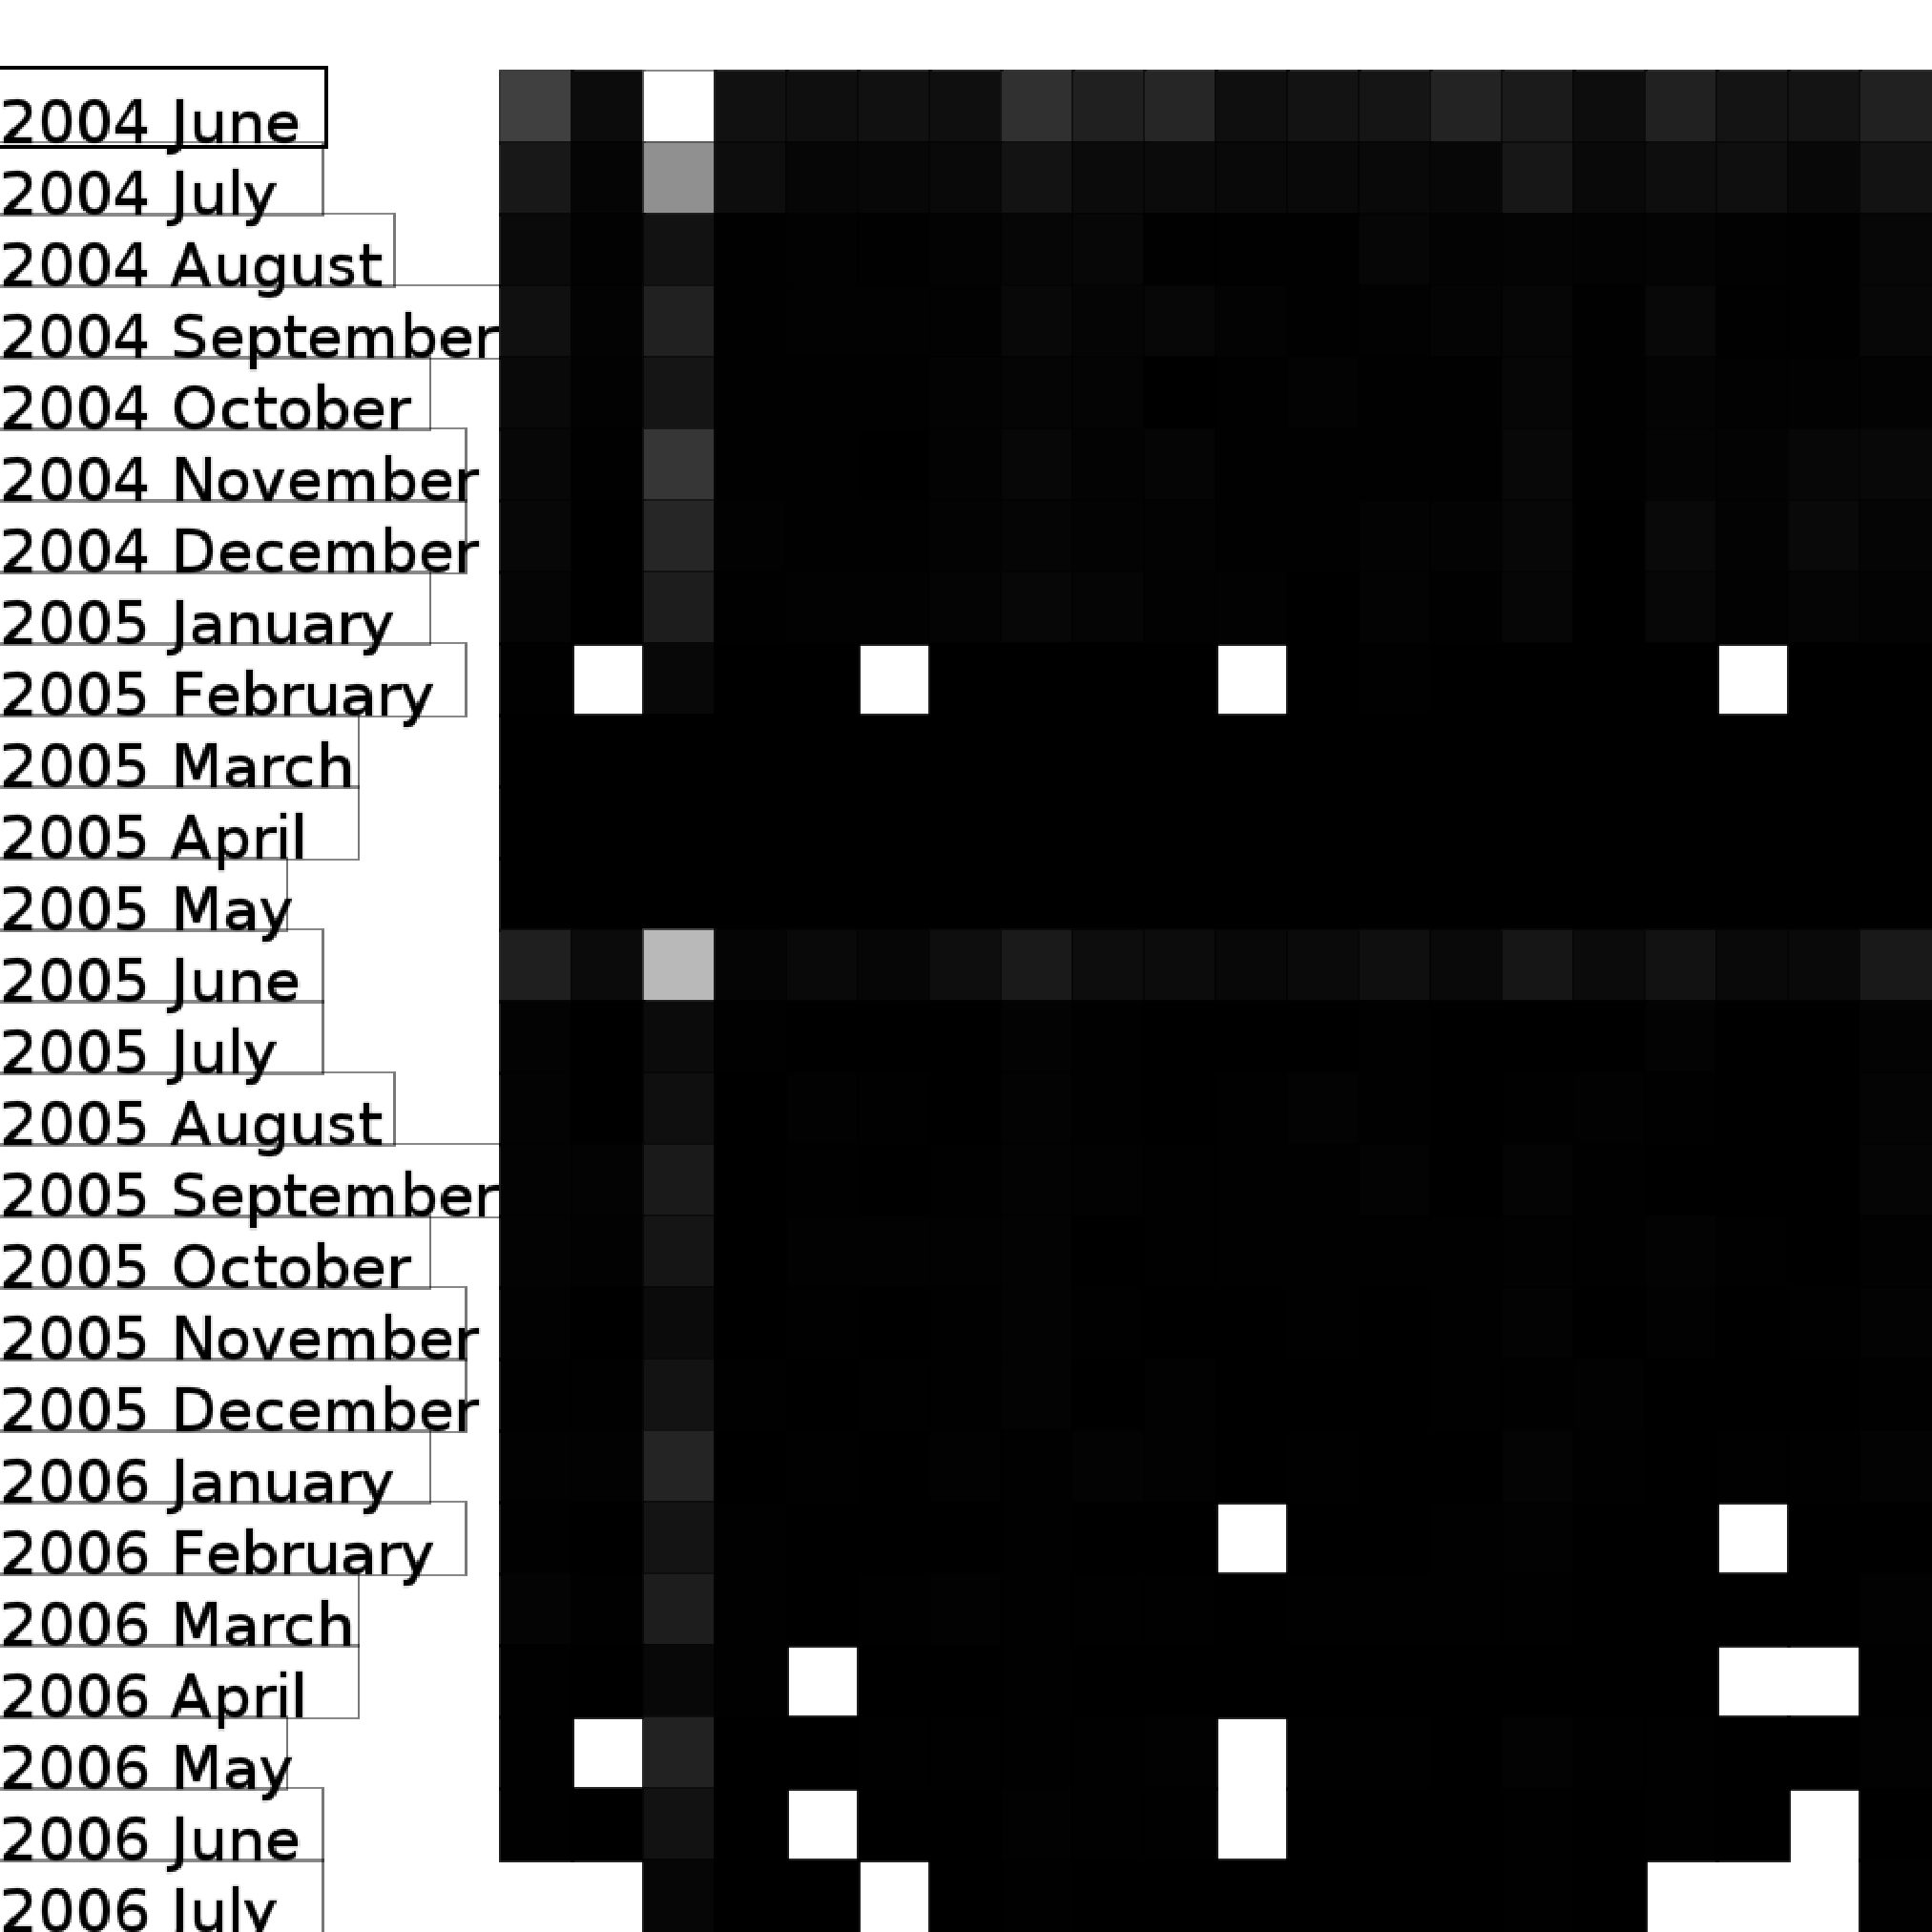
\includegraphics[width=0.45\textwidth]{month}
  \caption{MaxDB 7.500 topics analyzed with global topic analysis, 20
    topics (each row) and their document counts plotted over the
    entire development history of MaxDB 7.500 (26 months). The shade
    of the topic indicates the number of documents matching that topic
    in that month relative to the number of documents (white is most,
    black is least).}
  \label{fig:statictopics}
\end{figure}


%\SubSection{Validation}


%   1. well i'm stumped
%   2. look at it?
%   3. investigate those revisions and check the proportion etc
%   4. exploratory
%   5.   work it out
%8.   Validity Threats [0/5]
\shrinkit
\Section{Validity Threats}
\shrinkit

In this study we are explicitly trusting that the programmers annotate
their changes with relevant information. We rely on the descriptions
they provide. If the language of check-in comments was automated we
would  be analyzing only that.

We compared topics using the top 10 tokens, this approach could be
throwing data away and might not be as useful as determining the
actual distance between two word topic distributions.

% We truncated the topics to the top 10 tokens, so this summary of a topic
% might not have been as useful as determining the actual topic distance
% between two word topic distributions. By truncating tokens we could be
% losing valuable data.

Adding and removing stop words produced different results. Our choice
of stop words could be biased, and could affect the results.
%, and our bias for or against such stop words could affect
%the results.

% Each project seemed to have their own set of stop words, and we did not
% remove them, but perhaps dropping some of these stop words would aid
% the clarity of topics produced through topic analysis; alternatively
% it might cause our topic similarity plots to be fundamentally
% different.

The number of commits per month is inconsistent as some months have
many changes while other months have almost none.
%   1.   validation
%   2.   LDA is questionable
%   3.   blackbox problem
%   4.   not in the token
%   5.   multiple X token
%9.    Future Work

%10.   Conclusions



\shrinkit
\Section{Conclusions}
\shrinkit
%11.   Start file file:/home/abez/projects/lda-paper/lda-paper.tex


%XXX migod comments:

% The first two paras here are good stuff, but I think it belongs in
% section 5 at the end, as a summary of the utility of the approach.
% But can you add more meat to it in terms of numbers?


% In the conclusions you can simply restate what we did and what we
% learned without doing the arguing here.

% The third para is a good one for the conclusions, tho there need to
% be more detail.


We proposed and demonstrated the application of windowed topic
analysis, that is, topic analysis applied to commit messages during
periods of development. This approach differs from previous work that
applied topic analysis globally to the entire history of a
project without regard to time. We showed that many topics that exist
locally are relevant and interesting yet would often not be detected
via global topic analysis. We identify recurring topics with a topic
similarity measure that looks for topics which recur and mutate
repeatedly throughout the development of the software project.

Windowed topic analysis demonstrated its ability to hi-light local topics
and identify global trends. This was shown in our case study of MaxDB
7.500. Global topic analysis missed important topics such as
\emph{ODBC} while windowed topic analysis identified them.


We presented several visualization techniques that focused on
different aspects of the data: temporality of trends, trend size, and
a compact-trend-view. The compact-trend-view shows more
information than the views that global analysis could show, and it
indicates how focused a period is by the total number of topics. As
well, it shows topics by similarity so one can track trends across
time.  Our trend-histogram highlights and measures the
size of trends while our trend-time-line view shows how a topic
reoccurs over time. These visualizations help us  understand the common topics that developers focus on during
development. If implemented interactively an user could easily zoom in
and query for a summary of a topic or trend.
In summary, our work on windowed topic analysis shows the potential
for automatically determining key topics and trends across software
development projects .

\shrinkit
\SubSection{ Future Work}
\shrinkit
\shrinkit

\hla{ We want to explore parameters more across multiple projects,
  what motivates the need for more or less topics.  Parameters
  include: window overlapping, window overlap size, window size,
  number of topics, etc.  We want to investigate the effects of
  overlapping windows on this analysis. Do they make the trends too
  long? Do they highlight some trends unnecessarily or are they more
  because they are time agnostic.  }

Another avenue of future work is automatic topic labelling. Given a word
distribution we should be able to automatically select a word or term
that describes that distribution. Potential external sources of topic
names include: software engineering taxonomies, ontologies and
standards.


\shrinkit
\bibliographystyle{latex8}

\shrinkit
\bibliography{lda-paper}

%\bibliographystyle{abbrv}

% \Section{Appendix}

% \begin{itemize}
% \item We are missing a comparison of our technique to the classical technique
% \end{itemize}

\end{document}
